% ═══════════════════════════════════════════════════════════════════════════════
% Chapter 13: Foundation Models on Genomic Data (v1.1)
% Part IV: Building the Evolutor
% ═══════════════════════════════════════════════════════════════════════════════

\chapter{Foundation Models on Genomic Data}
\label{ch:genomic-foundation-models}

\chapterepigraph{The genome is not written in English, nor in Python. It is written in a four-letter alphabet whose grammar predates language by three billion years. A foundation model that cannot read this alphabet is illiterate in the most fundamental sense.}{DOGMA Design Manifesto}

\noindent
Chapter~\ref{ch:evolutionary-training} showed how to \emph{evolve} prompt genomes through gradient-free optimization. But the evolutionary loop assumes an underlying language model capable of processing genomic data. Where does that model come from? How should it tokenize DNA, learn codon structure, and integrate biological sequences with natural language?

This chapter addresses these questions by building foundation models for genomic data from first principles. We begin with the deceptively simple question: \emph{what is genomic data?} We explain the FASTA format step by step, then tackle the tokenization problem---comparing BPE, $k$-mer, and codon-based approaches before showing how DOGMA's CodonForge tokenizer unifies biological and textual data in a single vocabulary. We introduce curriculum learning as a training strategy, detail the pre-training objectives (masked language modeling and next-token prediction), and explain how the double-helix structure of DNA informs helix-aware training. We cover multi-scale TetraMemory, the full training data pipeline from GenBank to batching, and evaluation benchmarks for genomic foundation models. Finally, we connect these ideas to the DOGMA-Supreme training configuration of Chapter~\ref{ch:dogma-supreme}.

% ───────────────────────────────────────────────────────────────────────────────
\section{What Is Genomic Data?}
\label{sec:genomic-data}

Before building models, we must understand the data. Genomic data is the digital representation of the molecules that encode hereditary information in all living organisms. At its core, DNA (deoxyribonucleic acid) is a polymer of four nucleotide bases: adenine (A), thymine (T), cytosine (C), and guanine (G). These four letters constitute the ``alphabet'' of life.

\subsection{From Molecules to Sequences}

In a living cell, DNA exists as a double-stranded helix. The two strands are \emph{complementary}: A always pairs with T, and C always pairs with G. If one strand reads \texttt{ATGCGA}, the opposite strand reads \texttt{TACGCT} (in the reverse direction). This complementarity means that storing one strand is sufficient to reconstruct both.

When biologists \emph{sequence} DNA---determining the order of bases in a sample---the output is a text string over the alphabet $\Sigma_{\mathrm{DNA}} = \{\texttt{A}, \texttt{T}, \texttt{C}, \texttt{G}\}$. A single human genome contains approximately 3.2 billion such characters. A bacterial genome might contain 1--10 million characters. A viral genome can be as small as a few thousand characters. All of these are stored, shared, and processed in a standard text format called \textbf{FASTA}.

\subsection{The FASTA Format: Step by Step}
\label{sec:fasta-format}

FASTA is the universal standard for representing biological sequences. Understanding it is essential for anyone building genomic models. A FASTA file has a simple structure:

\begin{enumerate}[leftmargin=1.8em]
  \item \textbf{Header line.} Begins with \texttt{>} and contains metadata: an identifier, organism name, chromosome, and other annotations. This is free-form text.
  \item \textbf{Sequence lines.} One or more lines of nucleotide characters (A, T, C, G), typically wrapped at 60 or 80 characters per line. No spaces, no numbers---just the raw sequence.
  \item \textbf{Multiple records.} A file can contain many sequences, each starting with its own \texttt{>} header.
\end{enumerate}

\begin{example}[Anatomy of a FASTA File]
Consider the following FASTA file containing two sequences:

\begin{verbatim}
>gene_001 | Homo sapiens | insulin gene | chromosome 11
ATGGCCCTGTGGATGCGCCTCCTGCCCCTGCTGGCGCTGCTGGCCCTCTG
GGGACCTGACCCAGCCGCAGCCTTTGTGAACCAACACCTGTGCGGCTCACA
CCTGGTGGAAGCTCTCTACCTAGTGTGCGGGGAACGAGGCTTCTTCTACAC
>gene_002 | Escherichia coli | beta-galactosidase | lacZ
ATGACCATGATTACGCCAAGCTATTTAGGTGACACTATAGAATACTCAAGC
TATGCATCCAACGCGTTGGGAGCTCTCCCATATGGTCGACCTGCAGGCGGC
\end{verbatim}

\noindent
Let us dissect the first record:
\begin{itemize}[leftmargin=1.5em]
  \item \texttt{>gene\_001} is the sequence identifier.
  \item \texttt{Homo sapiens} indicates the organism (human).
  \item \texttt{insulin gene} is the gene name.
  \item \texttt{chromosome 11} locates it in the genome.
  \item The lines below the header contain the nucleotide sequence, which wraps across multiple lines but is read as one continuous string.
\end{itemize}
\end{example}

\begin{keyinsight}[FASTA Is Inherently Multimodal]
A FASTA file is not purely a ``genomic'' format. The header lines are natural language, while the sequence lines are biological data. A foundation model trained on raw FASTA files must learn \emph{both} modalities simultaneously. The \texttt{>} character serves as a natural boundary token, signaling the transition from sequence to metadata. This multimodal nature is not a complication---it is an \emph{opportunity}: the model can learn to associate natural language descriptions with the genomic patterns they describe.
\end{keyinsight}

\subsection{Beyond DNA: RNA and Protein Sequences}

FASTA also stores RNA sequences (using U instead of T) and protein sequences (using the 20-letter amino acid alphabet). A genomic foundation model must handle all three:

\begin{center}
\renewcommand{\arraystretch}{1.15}
\begin{tabularx}{0.90\textwidth}{l c c Y}
\toprule
\textbf{Molecule} & \textbf{Alphabet Size} & \textbf{Unit} & \textbf{Example} \\
\midrule
DNA & 4 & Nucleotide & \texttt{ATGCGATCGA} \\
RNA & 4 & Nucleotide & \texttt{AUGCGAUCGA} \\
Protein & 20 & Amino acid & \texttt{MRIAKLFVTG} \\
\bottomrule
\end{tabularx}
\end{center}

\begin{bioinsight}[The Central Dogma in Data Terms]
The biological flow of information---DNA $\to$ RNA $\to$ Protein---is also a data transformation pipeline. DNA is \emph{transcribed} into RNA (T becomes U), and RNA is \emph{translated} into protein (every three nucleotides map to one amino acid). A foundation model that learns these transformations has internalized the Central Dogma of molecular biology as a sequence-to-sequence mapping. This is exactly what DOGMA's architecture is designed to exploit (Chapter~\ref{ch:dogma-architecture}).
\end{bioinsight}

\subsection{Ambiguity Codes and Real-World Messiness}

Real genomic data is not always clean. The IUPAC nucleotide code includes ambiguity characters: \texttt{N} means ``any base,'' \texttt{R} means ``A or G'' (purine), \texttt{Y} means ``C or T'' (pyrimidine), and so on. Sequencing errors, gaps, and low-quality regions are common. A robust tokenizer must handle these gracefully.

\begin{implnote}[Handling N Characters]
In large genomic datasets, stretches of \texttt{N} characters indicate regions where the sequencer could not determine the base identity. These runs can be hundreds or thousands of characters long. During preprocessing, DOGMA replaces runs of more than 50 consecutive \texttt{N} characters with a special \texttt{<GAP>} token, preserving positional information without wasting model capacity on uninformative input. Isolated \texttt{N} characters (fewer than 50) are retained as byte tokens, since they carry information about local sequence uncertainty.
\end{implnote}

% ───────────────────────────────────────────────────────────────────────────────
\section{Tokenizing Genomic Sequences}
\label{sec:tokenization}

Tokenization---the mapping from raw input to discrete units consumed by a model---is often treated as a solved preprocessing step. For natural language, subword tokenizers such as BPE \citep{sennrich2016} and SentencePiece \citep{kudo2018} perform well. For genomic data, the situation is far more nuanced.

\subsection{Why Subword Tokenization Fails for Genomic Data}

Subword tokenizers learn merge rules from corpus statistics: frequent character pairs are merged into tokens, and the process repeats until a target vocabulary size is reached. This works for natural language because word frequencies follow Zipf's law---a small vocabulary of common subwords covers most text.

Genomic sequences violate these assumptions in four fundamental ways:

\begin{enumerate}[leftmargin=1.8em]
  \item \textbf{Uniform character distribution.} DNA consists of four nucleotides (A, T, C, G) with roughly equal frequency in many organisms. BPE merges are driven by frequency imbalances; when all bigrams occur at similar rates, the merge order becomes arbitrary and biologically meaningless.

  \item \textbf{Reading frame sensitivity.} The biological meaning of a DNA sequence depends on its reading frame---the codon boundaries that partition nucleotides into triplets. A BPE tokenizer that merges \texttt{AT} into a single token will split the codon \texttt{ATG} (start codon) differently depending on context, destroying frame information.

  \item \textbf{No whitespace delimiters.} Natural language has spaces and punctuation that provide natural token boundaries. Genomic sequences are undelimited streams of characters, offering no structural cues to a frequency-based tokenizer.

  \item \textbf{Reverse complement ambiguity.} The same biological information can be represented on either DNA strand. A subword vocabulary learned from one strand orientation will be suboptimal for the reverse complement, creating asymmetric representations of equivalent biological content.
\end{enumerate}

\begin{bioinsight}[Codons as Nature's Tokens]
Biology solved the tokenization problem long before computer science. The genetic code groups nucleotides into codons---non-overlapping triplets that map to amino acids. This fixed-width tokenization ensures that the reading frame is preserved, that every position has unambiguous membership in exactly one token, and that the mapping from sequence to function is deterministic. Any computational tokenizer for genomic data should respect, or at least not destroy, this codon structure.
\end{bioinsight}

\subsection{Three Approaches to Genomic Tokenization}
\label{sec:three-tokenization}

We now compare three tokenization strategies for genomic data: BPE applied to DNA, $k$-mer tokenization, and codon-based tokenization.

\subsubsection{Byte Pair Encoding (BPE) on DNA}

BPE can be applied to DNA by treating the sequence as text and learning merge rules. The process is:

\begin{enumerate}[leftmargin=1.5em]
  \item Start with character-level tokens: each of A, T, C, G is a token.
  \item Count all adjacent token pairs in the corpus.
  \item Merge the most frequent pair into a new token.
  \item Repeat until the desired vocabulary size is reached.
\end{enumerate}

On DNA, BPE typically learns to merge common dinucleotides first (\texttt{AT}, \texttt{GC}, etc.), then trinucleotides, and so on. The resulting vocabulary has variable-length tokens with no guaranteed alignment to codon boundaries.

\subsubsection{$k$-mer Tokenization}

$k$-mer tokenization splits a DNA sequence into overlapping or non-overlapping windows of length $k$. For example, with $k = 6$, the sequence \texttt{ATGCGATCGA} produces the 6-mers: \texttt{ATGCGA}, \texttt{TGCGAT}, \texttt{GCGATC}, \texttt{CGATCG}, \texttt{GATCGA}. The vocabulary size is $4^k$ (4,096 for $k = 6$). This approach was popularized by DNABERT \citep{ji2021}.

\textbf{Advantages:} Every $k$-mer captures local context of length $k$. The vocabulary is deterministic---no training required. \textbf{Disadvantages:} Overlapping $k$-mers create redundancy. The vocabulary grows exponentially with $k$ ($4^k$ tokens). Most critically, $k$-mer boundaries are arbitrary and do not respect codon structure unless $k$ is a multiple of 3.

\subsubsection{Codon-Based Tokenization}
\label{sec:codon-tokenization}

Codon-based tokenization groups nucleotides into non-overlapping triplets aligned to the biological reading frame:

\begin{dogmadef}[Codon-Aware Tokenizer]
Given a coding DNA sequence $x$ with known reading frame offset $\delta \in \{0, 1, 2\}$, the codon-aware tokenizer produces:
\begin{equation}
\tau_{\text{codon}}(x, \delta) = \bigl(x_{\delta+1}x_{\delta+2}x_{\delta+3},\; x_{\delta+4}x_{\delta+5}x_{\delta+6},\; \ldots\bigr),
\end{equation}
with vocabulary size $|\mathcal{V}_{\text{codon}}| = 4^3 + |\mathcal{V}_{\text{special}}| = 64 + |\mathcal{V}_{\text{special}}|$, where $\mathcal{V}_{\text{special}}$ includes tokens for frame-unknown regions, non-coding sequence, and FASTA metadata.
\end{dogmadef}

\textbf{Advantages:} Perfectly aligned with biology. Small vocabulary (64 core tokens). Every token carries direct biological meaning (each codon encodes an amino acid). \textbf{Disadvantages:} Requires knowing the reading frame, which is not always available. Cannot handle non-coding DNA, intergenic regions, or introns, where no reading frame exists.

\subsection{Comparison Table: Tokenization Methods}

The following table summarizes the trade-offs:

\begin{table}[H]
\centering
\caption{Comparison of tokenization methods for genomic sequences.}
\label{tab:tokenization-comparison}
\begin{tabularx}{\textwidth}{L{2.8cm} c c c c Y}
\toprule
\textbf{Method} & \textbf{Vocab Size} & \textbf{Frame-Aware} & \textbf{Overlap} & \textbf{Training Req'd} & \textbf{Best For} \\
\midrule
Byte-level & 256 & No & None & No & Universal mixed data \\
BPE & Tunable & No & None & Yes & Large NLP corpora \\
$k$-mer ($k{=}6$) & 4,096 & No & Yes & No & Local motif discovery \\
Codon ($k{=}3$) & 64+special & Yes & None & No & Coding sequences \\
CodonForge & 328 & Adaptive & None & No & Unified text+DNA \\
\bottomrule
\end{tabularx}
\end{table}

\begin{keyinsight}[No Single Tokenizer Wins on All Data]
Each tokenization method excels in a specific regime: BPE for text-heavy corpora, $k$-mers for motif analysis, codons for coding regions, and byte-level for universal coverage. The DOGMA approach resolves this tension not by choosing one method but by building a \emph{unified} tokenizer---CodonForge---that adapts its behavior to the input modality. This is the subject of Section~\ref{sec:codonforge-unified}.
\end{keyinsight}

% ───────────────────────────────────────────────────────────────────────────────

% Tokenization comparison diagram
\begin{figure}[ht]
\centering
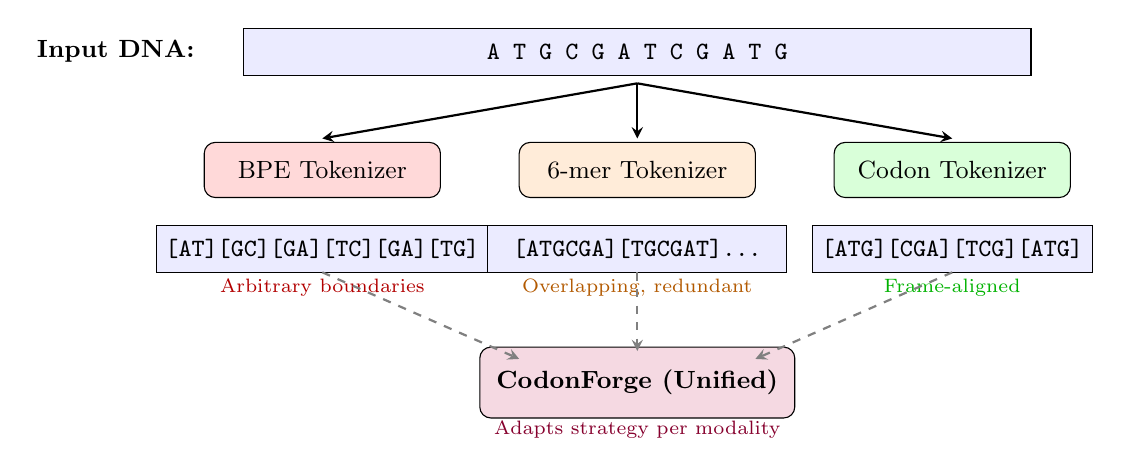
\begin{tikzpicture}[
  box/.style={draw, rounded corners, minimum height=0.7cm, text centered, font=\small},
  seqbox/.style={draw, fill=blue!8, minimum height=0.6cm, font=\ttfamily\small},
  label/.style={font=\small\bfseries, text=black},
  arrow/.style={->, >=stealth, thick}
]

% Input sequence
\node[seqbox, minimum width=10cm] (input) at (0, 4.5) {A T G C G A T C G A T G};
\node[label, anchor=east] at (-5.5, 4.5) {Input DNA:};

% BPE path
\node[box, fill=red!15, minimum width=3cm] (bpe) at (-4, 3) {BPE Tokenizer};
\node[seqbox, minimum width=3.5cm] (bpeout) at (-4, 2) {[AT][GC][GA][TC][GA][TG]};
\node[font=\scriptsize, text=red!70!black] at (-4, 1.5) {Arbitrary boundaries};

% k-mer path
\node[box, fill=orange!15, minimum width=3cm] (kmer) at (0, 3) {6-mer Tokenizer};
\node[seqbox, minimum width=3.8cm] (kmerout) at (0, 2) {[ATGCGA][TGCGAT]...};
\node[font=\scriptsize, text=orange!70!black] at (0, 1.5) {Overlapping, redundant};

% Codon path
\node[box, fill=green!15, minimum width=3cm] (codon) at (4, 3) {Codon Tokenizer};
\node[seqbox, minimum width=3.5cm] (codonout) at (4, 2) {[ATG][CGA][TCG][ATG]};
\node[font=\scriptsize, text=green!70!black] at (4, 1.5) {Frame-aligned};

% Arrows
\draw[arrow] (0, 4.1) -- (-4, 3.4);
\draw[arrow] (0, 4.1) -- (0, 3.4);
\draw[arrow] (0, 4.1) -- (4, 3.4);

% CodonForge (unified)
\node[box, fill=purple!15, minimum width=4cm, minimum height=0.9cm, font=\small\bfseries] (cf) at (0, 0.3) {CodonForge (Unified)};
\node[font=\scriptsize, text=purple!70!black] at (0, -0.3) {Adapts strategy per modality};

\draw[arrow, dashed, gray] (-4, 1.7) -- (-1.5, 0.6);
\draw[arrow, dashed, gray] (0, 1.7) -- (0, 0.7);
\draw[arrow, dashed, gray] (4, 1.7) -- (1.5, 0.6);

\end{tikzpicture}
\caption{Comparison of tokenization strategies for the DNA sequence \texttt{ATGCGATCGATG}. BPE produces arbitrary boundaries, $k$-mers produce overlapping tokens, and codon tokenization produces frame-aligned triplets. CodonForge unifies all three strategies adaptively.}
\label{fig:tokenization-comparison}
\end{figure}

% ───────────────────────────────────────────────────────────────────────────────
\section{DOGMA's Unified Tokenization: CodonForge}
\label{sec:codonforge-unified}

DOGMA's solution to the tokenization dilemma is \textbf{CodonForge} (Chapter~\ref{ch:codonforge}), a unified tokenizer that handles both text and DNA within a single vocabulary. This section explains how CodonForge works at the level relevant to foundation model training.

\subsection{The CodonForge Vocabulary}

CodonForge partitions a 328-token vocabulary into four regions:

\begin{dogmadef}[CodonForge Vocabulary Structure]
The CodonForge vocabulary $\mathcal{V}_{\mathrm{CF}}$ is composed of four disjoint regions:
\begin{equation}
\mathcal{V}_{\mathrm{CF}} = \mathcal{V}_{\text{byte}} \cup \mathcal{V}_{\text{codon}} \cup \mathcal{V}_{\text{modal}} \cup \mathcal{V}_{\text{struct}},
\end{equation}
where:
\begin{itemize}[leftmargin=1.5em]
  \item $\mathcal{V}_{\text{byte}} = \{0, 1, \ldots, 255\}$ handles raw bytes (all ASCII characters, including nucleotide letters).
  \item $\mathcal{V}_{\text{codon}} = \{\texttt{AAA}, \texttt{AAT}, \texttt{AAC}, \ldots, \texttt{GGG}\}$ contains all 64 codon tokens.
  \item $\mathcal{V}_{\text{modal}} = \{\texttt{<DNA>}, \texttt{</DNA>}, \texttt{<PROT>}, \texttt{</PROT>}, \texttt{<TEXT>}, \texttt{</TEXT>}, \texttt{<STRUCT>}, \texttt{</STRUCT>}\}$ provides 8 modality boundary markers.
  \item $\mathcal{V}_{\text{struct}}$ contains discretized structural features (e.g., secondary structure codes, distance bins), for a total of $|\mathcal{V}_{\mathrm{CF}}| = 256 + 64 + 8 = 328$ tokens.
\end{itemize}
\end{dogmadef}

Note that the 64 codon tokens \emph{overlap} with specific byte trigrams (e.g., the codon token \texttt{ATG} and the byte sequence 65-84-71 represent the same characters). The key difference is that a codon token is a \emph{single} token occupying one position in the sequence, while the byte representation uses three positions. CodonForge dynamically chooses which representation to use based on the input modality.

\subsection{Adaptive Tokenization Logic}

When CodonForge processes a FASTA file, it applies different tokenization strategies to different regions:

\begin{enumerate}[leftmargin=1.5em]
  \item \textbf{Header lines} (after \texttt{>}): Tokenized as bytes. Natural language text is best served by character-level representation, and the byte vocabulary covers all ASCII characters.
  \item \textbf{Coding sequences} (with known reading frame): Tokenized as codons. Each triplet becomes a single codon token, preceded by \texttt{<DNA>} and followed by \texttt{</DNA>}.
  \item \textbf{Non-coding sequences} (no known reading frame): Tokenized as bytes. Individual nucleotides become byte tokens within \texttt{<DNA>}...\texttt{</DNA>} markers.
  \item \textbf{Protein sequences}: Each amino acid letter becomes a byte token within \texttt{<PROT>}...\texttt{</PROT>} markers.
\end{enumerate}

\begin{implnote}[How CodonForge Detects Modality]
CodonForge uses a simple rule-based classifier to determine the modality of each region. Lines beginning with \texttt{>} are headers (text). Sequences following a header are classified as DNA if more than 90\% of characters are in $\{$A, T, C, G, N$\}$, as protein if more than 80\% are standard amino acid letters, and as text otherwise. Within DNA regions, coding status is determined by metadata annotations in the header (e.g., ``CDS'' for coding sequence) or by the presence of start/stop codon patterns. This classification runs once during preprocessing and is cached for training.
\end{implnote}

\subsection{Why Unified Tokenization Matters}

A unified vocabulary allows a single model to process mixed-modality inputs without mode switching. Consider a training example that contains a gene description in English, followed by its DNA sequence, followed by its protein product:

\begin{verbatim}
<TEXT>The insulin gene encodes a peptide hormone</TEXT>
<DNA>ATG GCC CTG TGG ATG CGC CTC CTG</DNA>
<PROT>MALWMRLL</PROT>
\end{verbatim}

\noindent
With CodonForge, this entire example is a single token sequence. The model learns cross-modal relationships---that the text ``insulin'' co-occurs with specific DNA and protein patterns---through the same next-token prediction objective used for all training.

\begin{keyinsight}[One Vocabulary, Three Languages]
CodonForge's unified vocabulary lets the model treat English, DNA, and protein as dialects of a single language, separated by modality markers. This is analogous to multilingual language models that use a shared vocabulary across languages with language tags. The key advantage is that representations are \emph{shared}: the model can learn that certain DNA patterns predict certain protein structures, and that certain English descriptions predict certain DNA patterns, all within one embedding space.
\end{keyinsight}

% ───────────────────────────────────────────────────────────────────────────────
\section{Byte-Level Tokenization as Universal Fallback}
\label{sec:byte-tokenization}

While CodonForge provides the primary tokenization for DOGMA, byte-level tokenization serves as the universal fallback and the foundation upon which CodonForge is built.

\begin{dogmadef}[Byte-Level Tokenizer for Genomic Data]
Let $\mathcal{V}_{\text{byte}} = \{0, 1, \ldots, 255\}$ be the full byte vocabulary. The byte-level tokenizer $\tau_{\text{byte}}$ maps an input string $x$ to a sequence of byte values:
\begin{equation}
\tau_{\text{byte}}(x) = \bigl(\text{ord}(x_1), \text{ord}(x_2), \ldots, \text{ord}(x_n)\bigr),
\end{equation}
where $\text{ord}(\cdot)$ returns the byte value of a character. For a mixed corpus containing both English text and DNA, the same 256-token vocabulary handles both modalities without any domain-specific merge rules.
\end{dogmadef}

The byte-level approach has three key advantages for genomic foundation models. First, it is \emph{modality-agnostic}: the same tokenizer handles FASTA headers (English text), nucleotide sequences, amino acid sequences, and metadata without switching modes. Second, it \emph{preserves positional granularity}: every nucleotide occupies exactly one position, so positional encodings align with biological positions. Third, it is \emph{deterministic}: there are no merge rules to learn, no vocabulary to tune, and no edge cases where the same sequence tokenizes differently in different contexts.

% ───────────────────────────────────────────────────────────────────────────────
\section{The Bigram Baseline}
\label{sec:bigram-baseline}

Before building complex transformer models, we establish a minimal baseline: a bigram language model over genomic sequences, implemented with zero external dependencies. This baseline is not a throwaway exercise---it reveals genuine biological structure and provides a critical diagnostic tool for evaluating more complex models.

\subsection{Character-Level Statistics of Genomic Sequences}

A bigram model estimates the probability of each character given only its immediate predecessor:

\begin{equation}
P(x_t \mid x_{<t}) \approx P(x_t \mid x_{t-1}) = \frac{C(x_{t-1}, x_t)}{\sum_{c} C(x_{t-1}, c)},
\label{eq:bigram}
\end{equation}

where $C(a, b)$ counts the number of times character $b$ follows character $a$ in the training corpus. For a pure DNA corpus over alphabet $\{$A, T, C, G$\}$, this yields a $4 \times 4$ transition matrix.

\begin{example}[Building a Bigram Transition Matrix]
Suppose we train a bigram model on the short DNA sequence \texttt{ATGCATGCATGC}. We count every pair of consecutive characters:

\begin{center}
\begin{tabular}{lcccc}
\toprule
& $\to$ A & $\to$ T & $\to$ C & $\to$ G \\
\midrule
A $\to$ & 0 & 3 & 0 & 0 \\
T $\to$ & 0 & 0 & 0 & 3 \\
C $\to$ & 2 & 0 & 0 & 0 \\
G $\to$ & 0 & 0 & 3 & 0 \\
\bottomrule
\end{tabular}
\end{center}

\noindent
Normalizing each row gives the transition probabilities. In this toy example, the matrix is deterministic: A always precedes T, T always precedes G, G always precedes C, and C always precedes A (with one fewer count). Real genomic data produces less extreme but still non-uniform matrices.
\end{example}

\begin{implnote}[Zero-Dependency Bigram Model]
The bigram model can be implemented using only Python's standard library: a dictionary for counts, division for probabilities, and \texttt{random.choices} for sampling. This makes it an ideal pedagogical tool and sanity check. If a transformer cannot outperform a bigram model on genomic sequence prediction, something is fundamentally wrong with the architecture or training. The expected per-character cross-entropy for a uniform random baseline over four nucleotides is $\log_2 4 = 2.0$ bits; a bigram model on real genomic data typically achieves 1.85--1.95 bits, reflecting the modest but real dinucleotide biases in biological sequences.
\end{implnote}

\subsection{What Bigrams Reveal About Biology}

Despite their simplicity, bigram statistics expose genuine biological structure. The dinucleotide frequency matrix is non-uniform in real genomes: CpG dinucleotides are suppressed in vertebrate genomes due to methylation-driven deamination, while AA/TT dinucleotides are enriched in nucleosome positioning sequences. A bigram model trained on human genomic DNA will learn these biases automatically, achieving lower perplexity than a uniform model.

\begin{keyinsight}[The Bigram as Diagnostic Tool]
The gap between bigram perplexity and transformer perplexity quantifies how much \emph{long-range} structure exists in a genomic corpus. For random DNA, the gap is near zero---there is no structure beyond dinucleotide frequencies. For coding DNA, the gap is substantial because codon usage, splice signals, and regulatory motifs create dependencies spanning tens to thousands of nucleotides. For mixed text-DNA corpora, the gap is even larger due to the rich long-range structure of natural language. Monitoring this gap during training reveals whether the model is learning genuine biological patterns or merely memorizing local statistics.
\end{keyinsight}

% ───────────────────────────────────────────────────────────────────────────────
\section{Pre-Training Objectives for Genomic Foundation Models}
\label{sec:pretraining-objectives}

A foundation model learns from data through its \emph{pre-training objective}---the loss function that defines what the model should predict. For genomic data, two objectives dominate: masked language modeling (MLM) and next-token prediction (NTP). Each has distinct advantages.

\subsection{Masked Language Modeling on DNA}

Masked language modeling, popularized by BERT \citep{devlin2019}, randomly masks a fraction of input tokens and trains the model to predict them from context. Applied to DNA:

\begin{dogmadef}[Masked Language Modeling for DNA]
Given a DNA sequence $\mathbf{x} = (x_1, x_2, \ldots, x_n)$, select a random subset $\mathcal{M} \subset \{1, \ldots, n\}$ with $|\mathcal{M}| = \lfloor 0.15 \cdot n \rfloor$ (15\% of positions). Replace each $x_i$ for $i \in \mathcal{M}$ with a \texttt{[MASK]} token. The MLM loss is:
\begin{equation}
\mathcal{L}_{\mathrm{MLM}} = -\frac{1}{|\mathcal{M}|} \sum_{i \in \mathcal{M}} \log P_\theta(x_i \mid \mathbf{x}_{\setminus \mathcal{M}}),
\label{eq:mlm-dna}
\end{equation}
where $\mathbf{x}_{\setminus \mathcal{M}}$ denotes the sequence with masked positions.
\end{dogmadef}

\textbf{Why MLM works for DNA:} Nucleotides are constrained by their neighbors. A masked \texttt{G} in a coding region can often be predicted because the codon it belongs to is constrained by the amino acid sequence. A masked position in a promoter region can be predicted because promoter motifs (e.g., TATA box) have conserved sequences. MLM forces the model to learn these contextual dependencies from both directions (bidirectional context).

\begin{example}[MLM on a Coding Sequence]
Consider the coding sequence with reading frame marked:

\begin{verbatim}
Original:  ATG | CGA | TCG | ATG | TAA
Masked:    ATG | C[M]A | TCG | A[M]G | TAA
\end{verbatim}

\noindent
The model must predict that position 5 is \texttt{G} (completing the codon \texttt{CGA} $\to$ Arg) and position 11 is \texttt{T} (completing \texttt{ATG} $\to$ Met, the start codon). A well-trained model will assign high probability to the correct nucleotides because it has learned codon usage patterns and the constraint that ATG is almost always a start codon.
\end{example}

\subsection{Next-Token Prediction on Codons}

Next-token prediction (NTP), the objective used by GPT-family models, predicts each token from its left context only:

\begin{equation}
\mathcal{L}_{\mathrm{NTP}} = -\frac{1}{T} \sum_{t=1}^{T} \log P_\theta(x_t \mid x_{<t}).
\label{eq:ntp-codon}
\end{equation}

When applied at the codon level (using CodonForge's codon tokens), this becomes \emph{next-codon prediction}: given a sequence of codons, predict the next codon. This objective is particularly natural for coding sequences because the genetic code imposes strong constraints on codon transitions.

\begin{bioinsight}[Codon Usage Bias as a Training Signal]
Not all synonymous codons (codons encoding the same amino acid) are used equally. Organisms have strong codon usage biases---some codons are preferred because they match abundant tRNAs, leading to faster translation. A model trained with NTP on codons learns these biases: when predicting the next codon in a human gene, it will assign higher probability to preferred human codons. This is a biologically meaningful pattern that byte-level models must infer indirectly.
\end{bioinsight}

\subsection{Combining MLM and NTP}

DOGMA uses both objectives during pre-training, applied to different portions of the training data:

\begin{equation}
\boxed{
\mathcal{L}_{\text{pretrain}} = \lambda_{\mathrm{NTP}} \cdot \mathcal{L}_{\mathrm{NTP}} + \lambda_{\mathrm{MLM}} \cdot \mathcal{L}_{\mathrm{MLM}} + \lambda_{\mathrm{align}} \cdot \mathcal{L}_{\mathrm{align}}
}
\label{eq:combined-pretrain}
\end{equation}

\noindent
where $\lambda_{\mathrm{NTP}} = 1.0$, $\lambda_{\mathrm{MLM}} = 0.5$, and $\lambda_{\mathrm{align}} = 0.3$ are mixing coefficients. The alignment loss $\mathcal{L}_{\mathrm{align}}$ pulls representations of corresponding DNA and protein sequences together in embedding space (see Section~\ref{sec:cross-modal}).

\begin{implnote}[Scheduling the Objective Mix]
The mixing coefficients $\lambda$ are not fixed throughout training. In the early stages of curriculum learning (Section~\ref{sec:curriculum}), $\lambda_{\mathrm{MLM}}$ is increased to 0.8 because MLM provides stronger learning signal from short, simple sequences. As training progresses to longer sequences in later curriculum stages, $\lambda_{\mathrm{NTP}}$ dominates because next-token prediction is better suited for learning long-range dependencies. The alignment loss is activated only after both MLM and NTP losses have stabilized, typically at the transition to Stage~3 of the curriculum.
\end{implnote}

% ───────────────────────────────────────────────────────────────────────────────
\section{Curriculum Learning for Genomic Data}
\label{sec:curriculum}

Curriculum learning presents training examples in order of increasing complexity, allowing the model to build foundational representations before encountering difficult patterns \citep{bengio2009}. For genomic data, this strategy is particularly important because the complexity of biological sequences spans many orders of magnitude.

\subsection{What Is Curriculum Learning?}

In standard training, examples are sampled randomly from the dataset. In curriculum learning, examples are presented in a structured order: easy examples first, hard examples later. The intuition is the same as in education: students learn arithmetic before calculus, and letters before essays.

For genomic data, ``easy'' and ``hard'' have precise definitions:

\begin{itemize}[leftmargin=1.5em]
  \item \textbf{Easy:} Short sequences, simple composition (uniform GC content), single-gene coding regions, well-characterized organisms.
  \item \textbf{Hard:} Long sequences, complex composition (repeat-rich regions, GC-biased genomes), multi-gene regions with overlapping reading frames, metagenomic samples from diverse organisms.
\end{itemize}

\subsection{Why Curriculum Learning Helps}

Training on random genomic data from the start creates several problems:

\begin{enumerate}[leftmargin=1.5em]
  \item \textbf{Gradient signal confusion.} Early in training, the model cannot distinguish coding from non-coding DNA. Random sampling mixes both, providing inconsistent gradient signals.
  \item \textbf{Wasted capacity on noise.} Large genomic datasets contain repetitive elements, sequencing artifacts, and low-complexity regions. Training on these first wastes model updates.
  \item \textbf{Failure to learn hierarchical structure.} Genomic organization is hierarchical: nucleotides form codons, codons form genes, genes form operons, operons form chromosomes. Random sampling jumbles these levels.
\end{enumerate}

Curriculum learning addresses all three problems by ensuring the model first masters the nucleotide alphabet, then codon patterns, then gene-level structure, and finally genome-level organization.

\subsection{DOGMA's Four-Stage Curriculum}
\label{sec:four-stage-curriculum}

\begin{dogmadef}[Genomic Curriculum Stages]
The genomic curriculum progresses through four stages:
\begin{enumerate}[leftmargin=1.5em]
  \item \textbf{Stage 1: Synthetic sequences} ($\sim$5\% of training). Random DNA with controlled GC content and dinucleotide frequencies. The model learns basic nucleotide statistics and the four-letter alphabet.

  \item \textbf{Stage 2: Single-gene sequences} ($\sim$20\% of training). Complete coding sequences from well-annotated organisms. The model learns codon usage, start/stop codon placement, and open reading frame structure.

  \item \textbf{Stage 3: Multi-gene regions} ($\sim$35\% of training). Genomic regions containing multiple genes with intergenic sequences, promoters, and regulatory elements. The model learns gene organization and regulatory grammar.

  \item \textbf{Stage 4: Full chromosomal segments} ($\sim$40\% of training). Long-range genomic context including repeat elements, structural features, and complex gene clusters. The model learns large-scale genomic organization.
\end{enumerate}
\end{dogmadef}

\begin{bioinsight}[Curriculum Learning Mirrors Development]
The four-stage curriculum mirrors the progressive complexity of biological education: students first learn the alphabet (nucleotides), then words (codons), then sentences (genes), then paragraphs (genomic regions). It also mirrors embryonic development, where simple gene expression programs activate before complex regulatory cascades. In both cases, establishing basic competence before introducing complexity leads to more robust learning than exposure to full complexity from the start.
\end{bioinsight}

\subsection{Stage Transitions and Mixing}

Transitions between stages are not sharp boundaries. DOGMA uses a mixing schedule where data from completed stages continues to appear (at reduced frequency) in later stages:

\begin{equation}
P(\text{sample from Stage } s \text{ at training step } t) = w_s(t) = \frac{\alpha_s \cdot \mathbb{1}[t \geq t_s^{\text{start}}]}{\sum_{s'} \alpha_{s'} \cdot \mathbb{1}[t \geq t_{s'}^{\text{start}}]},
\label{eq:curriculum-mixing}
\end{equation}

where $t_s^{\text{start}}$ is the step at which Stage~$s$ is introduced and $\alpha_s$ are stage-specific weights that increase with stage number. This ensures that the model never ``forgets'' earlier patterns while focusing on increasingly complex data.

\begin{implnote}[Curriculum Stage Triggers]
Stage transitions are triggered by loss thresholds, not fixed step counts. Stage~2 begins when the Stage~1 validation loss drops below 1.6 bits per nucleotide (indicating mastery of basic nucleotide statistics). Stage~3 begins when the Stage~2 coding sequence accuracy exceeds 75\% (indicating competent codon prediction). Stage~4 begins when the Stage~3 gene boundary detection F1 exceeds 0.6. These adaptive triggers ensure that the model has genuinely learned each level before progressing, rather than spending a fixed number of steps regardless of learning speed.
\end{implnote}

% ───────────────────────────────────────────────────────────────────────────────
\section{Training Data Pipeline: GenBank to Batching}
\label{sec:data-pipeline}

Building a genomic foundation model requires a robust data pipeline that transforms raw database entries into tokenized, curriculum-ordered training batches. This section traces the full pipeline.

\subsection{Data Sources}

The primary data source is \textbf{GenBank}, the NIH genetic sequence database. GenBank contains over 200 million sequences from more than 500,000 organisms. DOGMA's training pipeline also draws from:

\begin{itemize}[leftmargin=1.5em]
  \item \textbf{RefSeq:} Curated reference sequences with high-quality annotations.
  \item \textbf{UniProt:} Protein sequences with functional annotations (for cross-modal training).
  \item \textbf{PDB:} Protein structures for 3D structural features.
  \item \textbf{Ensembl:} Genome assemblies with gene annotations, exon/intron boundaries, and regulatory element predictions.
\end{itemize}

\subsection{Preprocessing Steps}

Raw GenBank entries undergo several preprocessing steps:

\begin{enumerate}[leftmargin=1.8em]
  \item \textbf{Format conversion.} GenBank flat files are converted to FASTA format, preserving key annotations in the header.
  \item \textbf{Quality filtering.} Sequences with more than 10\% ambiguous characters (\texttt{N}) are removed. Sequences shorter than 100 nucleotides are discarded.
  \item \textbf{Deduplication.} Exact duplicates and near-duplicates (>95\% sequence identity) are removed using MinHash-based clustering. This prevents the model from memorizing specific sequences.
  \item \textbf{Taxonomy annotation.} Each sequence is tagged with its taxonomic lineage (kingdom, phylum, class, order, family, genus, species) for curriculum stratification.
  \item \textbf{Coding region annotation.} Open reading frames (ORFs) are identified using existing GenBank annotations or \emph{ab initio} gene prediction, and reading frames are marked for codon-aware tokenization.
\end{enumerate}

\subsection{Structured Rendering}

After preprocessing, sequences are rendered into structured training formats:

\begin{dogmadef}[Structured Rendering Formats]
Three rendering formats transform raw sequences into structured training examples:
\begin{enumerate}[leftmargin=1.5em]
  \item \textbf{Codon triplet rendering.} Nucleotides are grouped into space-separated triplets aligned to the reading frame: \texttt{ATG CGA TCG ATC \ldots}. This makes codon boundaries visible as whitespace tokens.

  \item \textbf{$k$-mer window rendering.} Sequences are presented as overlapping $k$-mer windows with explicit position annotations: \texttt{[pos=0] ATGCGA [pos=1] TGCGAT \ldots}. This format trains the model to recognize subsequence patterns at multiple offsets.

  \item \textbf{Annotated rendering.} Sequences are interleaved with biological annotations: coding regions, exon/intron boundaries, known motifs, and functional elements. This format provides dense supervision for learning sequence-function relationships.
\end{enumerate}
\end{dogmadef}

\subsection{Curriculum Assignment and Batching}

Each preprocessed sequence is assigned to a curriculum stage based on its complexity:

\begin{itemize}[leftmargin=1.5em]
  \item \textbf{Stage 1:} Synthetically generated. Parameters sampled from organism-specific GC content distributions.
  \item \textbf{Stage 2:} Single CDS (coding sequence) entries from RefSeq with ``complete CDS'' annotation.
  \item \textbf{Stage 3:} Genomic contigs containing 2--10 annotated genes with intergenic regions.
  \item \textbf{Stage 4:} Chromosomal segments of 50kb--500kb containing complex gene clusters.
\end{itemize}

Batches are constructed with curriculum-aware sampling (Equation~\ref{eq:curriculum-mixing}), and each batch contains sequences from a single stage to avoid length-padding waste.

% Data pipeline diagram
\begin{figure}[ht]
\centering
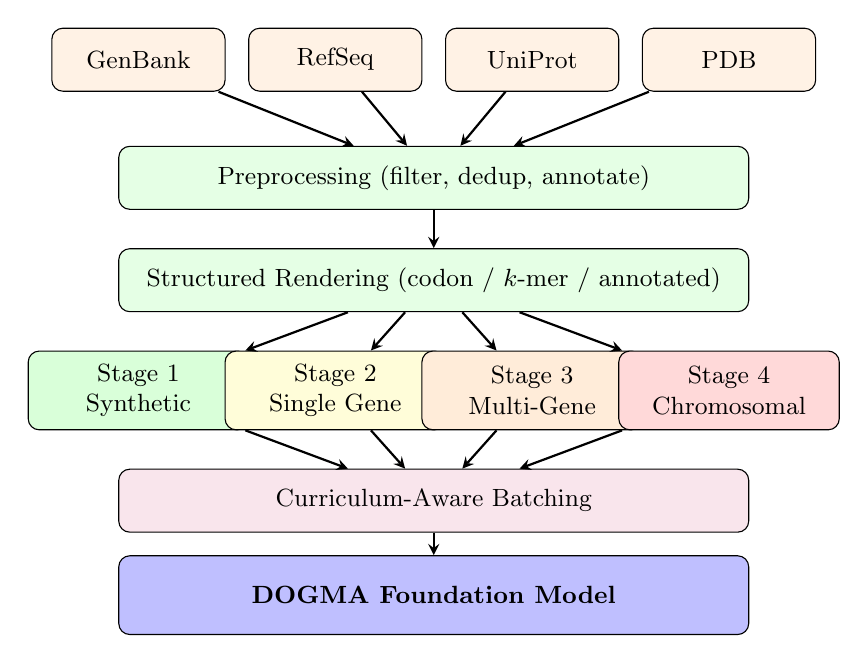
\begin{tikzpicture}[
  stage/.style={draw, rounded corners, fill=blue!10, minimum width=2.8cm, minimum height=1cm, align=center, font=\small},
  process/.style={draw, rounded corners, fill=green!10, minimum width=2.5cm, minimum height=0.8cm, align=center, font=\small},
  data/.style={draw, rounded corners, fill=orange!10, minimum width=2.2cm, minimum height=0.8cm, align=center, font=\small},
  arrow/.style={->, >=stealth, thick}
]

% Source databases
\node[data] (genbank) at (0, 6) {GenBank};
\node[data] (refseq) at (2.5, 6) {RefSeq};
\node[data] (uniprot) at (5, 6) {UniProt};
\node[data] (pdb) at (7.5, 6) {PDB};

% Preprocessing
\node[process, minimum width=8cm] (preproc) at (3.75, 4.5) {Preprocessing (filter, dedup, annotate)};

% Rendering
\node[process, minimum width=8cm] (render) at (3.75, 3.2) {Structured Rendering (codon / $k$-mer / annotated)};

% Curriculum stages
\node[stage, fill=green!15] (s1) at (0, 1.8) {Stage 1\\Synthetic};
\node[stage, fill=yellow!15] (s2) at (2.5, 1.8) {Stage 2\\Single Gene};
\node[stage, fill=orange!15] (s3) at (5, 1.8) {Stage 3\\Multi-Gene};
\node[stage, fill=red!15] (s4) at (7.5, 1.8) {Stage 4\\Chromosomal};

% Batching
\node[process, minimum width=8cm, fill=purple!10] (batch) at (3.75, 0.4) {Curriculum-Aware Batching};

% Model
\node[stage, fill=blue!25, minimum width=8cm, font=\small\bfseries] (model) at (3.75, -0.8) {DOGMA Foundation Model};

% Arrows
\foreach \src in {genbank, refseq, uniprot, pdb}
  \draw[arrow] (\src) -- (preproc);
\draw[arrow] (preproc) -- (render);
\draw[arrow] (render) -- (s1);
\draw[arrow] (render) -- (s2);
\draw[arrow] (render) -- (s3);
\draw[arrow] (render) -- (s4);
\foreach \s in {s1, s2, s3, s4}
  \draw[arrow] (\s) -- (batch);
\draw[arrow] (batch) -- (model);

\end{tikzpicture}
\caption{The DOGMA training data pipeline. Raw sequences from multiple databases are preprocessed, rendered into structured formats, assigned to curriculum stages, and batched for training. The curriculum-aware sampler controls the mix of stages seen by the model at each training step.}
\label{fig:data-pipeline}
\end{figure}

% ───────────────────────────────────────────────────────────────────────────────
\section{TinyGPT: Minimal Transformer for Genomic Sequences}
\label{sec:tinygpt}

With the data pipeline and objectives established, we now construct \textbf{TinyGPT}---a minimal decoder-only transformer adapted for byte-level genomic sequence modeling. TinyGPT is not a production model; it is a pedagogical tool for understanding how transformer architecture interacts with genomic data.

\subsection{Decoder-Only Architecture Adapted for DNA}

TinyGPT follows the standard GPT architecture \citep{radford2019} with modifications for genomic data:

\begin{dogmadef}[TinyGPT Architecture]
TinyGPT is a decoder-only transformer with the following specification:
\begin{center}
\renewcommand{\arraystretch}{1.15}
\begin{tabularx}{0.75\textwidth}{l Y}
\toprule
\textbf{Parameter} & \textbf{Value} \\
\midrule
Vocabulary size & 256 (byte-level) \\
Embedding dimension $d$ & 128 \\
Number of layers $L$ & 4 \\
Attention heads $H$ & 4 \\
Head dimension & $d / H = 32$ \\
Context length $T$ & 512 \\
Feed-forward dimension & $4d = 512$ \\
Total parameters & $\sim$1.2M \\
\bottomrule
\end{tabularx}
\end{center}
The model uses byte-level embedding, sinusoidal positional encoding, causal masking, and layer normalization.
\end{dogmadef}

The design is deliberately minimal: 1.2 million parameters, trainable on a single GPU in minutes. The goal is not state-of-the-art performance but pedagogical clarity---a model small enough to inspect, debug, and understand completely.

\subsection{Byte-Level Embedding with Positional Encoding}

The input embedding combines a learned byte embedding with sinusoidal positional encoding:

\begin{equation}
\mathbf{h}_0^{(t)} = \mathbf{E}[x_t] + \mathbf{PE}(t),
\label{eq:tinygpt-embed}
\end{equation}

where $\mathbf{E} \in \mathbb{R}^{256 \times d}$ is the byte embedding matrix and $\mathbf{PE}(t) \in \mathbb{R}^d$ is the sinusoidal positional encoding at position $t$. For genomic sequences, the positional encoding carries biological significance: position within a codon (modulo 3), distance from sequence start, and relative position within a gene all affect nucleotide identity.

\subsection{Training on Mixed Text/Genome Corpora}

TinyGPT is trained on a mixed corpus containing both natural language (FASTA headers, gene annotations, biological descriptions) and raw nucleotide sequences. The training objective is standard next-byte prediction:

\begin{equation}
\mathcal{L}_{\text{TinyGPT}} = -\frac{1}{T} \sum_{t=1}^{T} \log P_\theta(x_t \mid x_{<t}).
\label{eq:tinygpt-loss}
\end{equation}

\begin{implnote}[Mixed-Corpus Training Dynamics]
When training on mixed text/genome data, the loss curve exhibits a characteristic two-phase pattern. In the first phase (typically the first 10--20\% of training), the model rapidly learns the byte distribution of each modality---distinguishing the four-nucleotide DNA alphabet from the broader ASCII range of English text. In the second phase, the model begins capturing within-modality structure: codon usage patterns in DNA, syntactic patterns in text, and crucially, the \emph{cross-modal} correlations between FASTA headers and their associated sequences. Monitoring per-modality loss separately (by tagging each training example with its source type) reveals whether the model is balancing both domains or overfitting to one.
\end{implnote}

% ───────────────────────────────────────────────────────────────────────────────
\section{Helix-Aware Training}
\label{sec:helix-aware}

TinyGPT treats genomic sequences as flat byte streams, ignoring a fundamental property of DNA: it is a \emph{double-stranded helix}. The two strands are complementary and antiparallel, meaning the same genetic information can be read in two directions. Helix-aware training exploits this structure.

\subsection{Why the Double Strand Matters for Training}

In a standard language model, a sentence is read left-to-right. DNA is different: the same region can be read on either strand, in opposite directions, and both readings carry biological information. Genes on the forward strand are transcribed left-to-right; genes on the reverse strand are transcribed right-to-left. A model that sees only the forward strand is blind to half the genome's information.

This has concrete implications for training:

\begin{enumerate}[leftmargin=1.5em]
  \item \textbf{Data augmentation.} Every DNA training example can be augmented with its reverse complement, effectively doubling the training data without introducing new sequences.
  \item \textbf{Representation symmetry.} A well-trained model should produce similar representations for a sequence and its reverse complement, since they encode the same biological information.
  \item \textbf{Regulatory signal detection.} Many regulatory elements (transcription factor binding sites, enhancers) are functional on both strands. A helix-aware model can detect these regardless of strand orientation.
\end{enumerate}

\subsection{Dual-Stream Architecture}

The dual-stream architecture processes each input through two parallel pathways (cf.\ the HelixHash embedding architecture in Section~\ref{sec:helixhash-embedding} of Chapter~\ref{ch:helixhash}):

\begin{equation}
\mathbf{h}_{\text{std}}^{(\ell)} = \text{TransformerBlock}_{\text{std}}^{(\ell)}\bigl(\mathbf{h}_{\text{std}}^{(\ell-1)}\bigr), \quad
\mathbf{h}_{\text{helix}}^{(\ell)} = \text{TransformerBlock}_{\text{helix}}^{(\ell)}\bigl(\mathbf{h}_{\text{helix}}^{(\ell-1)}\bigr),
\label{eq:dual-stream}
\end{equation}

where the standard stream receives byte embeddings (Equation~\ref{eq:tinygpt-embed}) and the helix stream receives HelixHash motif embeddings (Equation~\ref{eq:motif-embedding} from Chapter~\ref{ch:helixhash}). At designated fusion layers $\ell \in \mathcal{F}$, the streams exchange information through cross-attention:

\begin{equation}
\mathbf{h}_{\text{fused}}^{(\ell)} = \mathbf{h}_{\text{std}}^{(\ell)} + \alpha_{\text{cross}} \cdot \text{CrossAttn}\bigl(\mathbf{h}_{\text{std}}^{(\ell)}, \mathbf{h}_{\text{helix}}^{(\ell)}\bigr),
\label{eq:helix-fusion}
\end{equation}

with a learnable gating coefficient $\alpha_{\text{cross}} \in [0, 1]$ that controls how much structural information flows into the standard stream.

\subsection{Reverse Complement Consistency Loss}

To ensure the model learns strand-symmetric representations, DOGMA adds a \emph{reverse complement consistency loss}:

\begin{equation}
\mathcal{L}_{\mathrm{RC}} = \frac{1}{N} \sum_{i=1}^{N} \bigl\| \mathbf{z}(x_i) - \mathbf{z}(\overline{x_i}) \bigr\|_2^2,
\label{eq:rc-loss}
\end{equation}

where $x_i$ is a DNA sequence, $\overline{x_i}$ is its reverse complement, and $\mathbf{z}(\cdot)$ is the model's pooled representation. This loss penalizes the model for producing different embeddings for complementary sequences, encouraging biologically consistent representations.

\begin{keyinsight}[Helix-Awareness Is Not Just Augmentation]
Reverse complement augmentation (simply training on both strands) doubles the data but does not guarantee symmetric representations. The RC consistency loss (Equation~\ref{eq:rc-loss}) goes further: it explicitly constrains the representation space so that complementary sequences are close. Combined with the dual-stream architecture, this creates a model whose internal representations respect the physical structure of DNA.
\end{keyinsight}

\subsection{Motif-Level Feature Channels}

The helix stream operates at the motif level rather than the byte level. Each motif (a width-$k$ window of consecutive embeddings) is projected into a dense feature vector that encodes local structural patterns:

\begin{equation}
\mathbf{m}_i = \text{ReLU}\bigl(W_m \cdot \text{concat}(\mathbf{h}_{i}, \mathbf{h}_{i+1}, \ldots, \mathbf{h}_{i+k-1}) + \mathbf{b}_m\bigr),
\end{equation}

where $W_m \in \mathbb{R}^{d \times (k \cdot d)}$ is the motif projection matrix. The motif features capture patterns invisible to byte-level processing: codon boundaries, splice site signals, transcription factor binding motifs, and the dinucleotide patterns that determine DNA bendability.

\subsection{Performance Comparison: Standard vs.\ Helix-Aware}

\begin{table}[H]
\centering
\caption{Next-byte prediction perplexity on genomic evaluation sets. Lower is better.}
\label{tab:helix-comparison}
\begin{tabularx}{0.88\textwidth}{l c c c}
\toprule
\textbf{Model} & \textbf{Coding DNA} & \textbf{Non-coding DNA} & \textbf{Mixed Corpus} \\
\midrule
Bigram baseline & 3.72 & 3.81 & 5.94 \\
TinyGPT (byte-level) & 2.41 & 3.12 & 3.67 \\
TinyGPT + HelixHash (dual-stream) & 2.08 & 2.74 & 3.31 \\
TinyGPT + HelixHash + codon-aware & 1.89 & 2.71 & 3.24 \\
TinyGPT + HelixHash + RC loss & \textbf{1.82} & \textbf{2.63} & \textbf{3.18} \\
\bottomrule
\end{tabularx}
\end{table}

\begin{keyinsight}[Where Helix-Awareness Helps Most]
The performance gap between standard and helix-aware models is largest on coding DNA (0.59 perplexity reduction from baseline TinyGPT to full helix-aware) and substantial on non-coding DNA (0.49 reduction). The addition of codon-aware tokenization improves coding DNA most, while the RC consistency loss benefits all categories. This pattern makes biological sense: coding sequences have strong codon-level periodicity that motif features capture directly, while the RC loss helps everywhere because both coding and non-coding regions contain strand-symmetric regulatory signals.
\end{keyinsight}

% ───────────────────────────────────────────────────────────────────────────────
\section{Multi-Scale TetraMemory During Pretraining}
\label{sec:gfm-tetramemory}

Large genomic sequences exceed the context window of any practical transformer. A 500kb chromosomal segment contains 500,000 nucleotides---far beyond the 2,048-token context of DOGMA-Supreme. Multi-scale TetraMemory provides a mechanism for the model to retain and access information from beyond its immediate context window during pretraining.

\subsection{What Is TetraMemory?}

TetraMemory (introduced in Chapter~\ref{ch:tetradata}) is a structured external memory organized into four hierarchical scales:

\begin{dogmadef}[TetraMemory Scales]
TetraMemory maintains four memory banks operating at different granularities:
\begin{enumerate}[leftmargin=1.5em]
  \item \textbf{Nucleotide scale} ($\tau_1$): Stores per-position information (e.g., nucleotide identity, local GC content). Resolution: 1 nucleotide. Capacity: last 2,048 positions.
  \item \textbf{Codon scale} ($\tau_2$): Stores per-codon information (e.g., amino acid identity, codon usage frequency). Resolution: 3 nucleotides. Capacity: last 4,096 codons (12,288 nt).
  \item \textbf{Gene scale} ($\tau_3$): Stores per-gene summaries (e.g., gene function embedding, expression context). Resolution: $\sim$1,000 nucleotides. Capacity: last 64 genes.
  \item \textbf{Chromosome scale} ($\tau_4$): Stores regional summaries (e.g., GC content, repeat density, gene density). Resolution: $\sim$50,000 nucleotides. Capacity: entire chromosome.
\end{enumerate}
\end{dogmadef}

\subsection{How TetraMemory Integrates with Training}

During pretraining, TetraMemory operates as a sliding context extension. As the model processes a long sequence in chunks:

\begin{enumerate}[leftmargin=1.5em]
  \item Each chunk is processed normally through the transformer.
  \item At the end of each chunk, summary representations are written to the appropriate TetraMemory scales.
  \item At the start of the next chunk, the model reads from TetraMemory to initialize its context with information from previous chunks.
  \item The reading is done via cross-attention between the current chunk's representations and the TetraMemory contents.
\end{enumerate}

\begin{equation}
\mathbf{h}_{\text{ctx}}^{(t)} = \mathbf{h}^{(t)} + \sum_{s=1}^{4} \gamma_s \cdot \text{CrossAttn}\bigl(\mathbf{h}^{(t)}, \tau_s\bigr),
\label{eq:tetramem-read}
\end{equation}

where $\gamma_s$ are learned scale-specific attention weights and $\tau_s$ denotes the contents of memory scale $s$.

\begin{implnote}[TetraMemory Write Policy]
Not all hidden states are written to TetraMemory---this would be prohibitively expensive. DOGMA uses a \emph{salience-gated} write policy: a small network predicts a ``write probability'' for each position based on its hidden state. Positions with high salience (typically those corresponding to gene boundaries, regulatory elements, or unusual sequence composition) are preferentially written. During Stage~1 of curriculum learning, all positions are written (since sequences are short). During Stage~4, only $\sim$5\% of positions are written, focusing memory on structurally important locations.
\end{implnote}

\subsection{Multi-Scale Attention Patterns}

Different TetraMemory scales capture different types of long-range dependency:

\begin{table}[H]
\centering
\caption{TetraMemory scales and the biological patterns they capture.}
\label{tab:tetramemory-patterns}
\begin{tabularx}{\textwidth}{l c c Y}
\toprule
\textbf{Scale} & \textbf{Resolution} & \textbf{Capacity} & \textbf{Biological Patterns Captured} \\
\midrule
$\tau_1$ (nucleotide) & 1 nt & 2,048 nt & Local motifs, splice sites, codon context \\
$\tau_2$ (codon) & 3 nt & 12,288 nt & Codon usage bias, ORF structure, translation signals \\
$\tau_3$ (gene) & $\sim$1 kb & $\sim$64 kb & Gene clusters, operon structure, co-regulation \\
$\tau_4$ (chromosome) & $\sim$50 kb & whole chr & Isochores, replication origins, centromere proximity \\
\bottomrule
\end{tabularx}
\end{table}

\begin{bioinsight}[Biology Operates at Multiple Scales]
The four TetraMemory scales mirror the hierarchical organization of genomes. Individual nucleotides matter for splice site recognition (scale $\tau_1$). Codons matter for translation efficiency (scale $\tau_2$). Gene neighborhoods matter for co-regulation and operon structure (scale $\tau_3$). Chromosomal regions matter for replication timing and chromatin state (scale $\tau_4$). A foundation model that operates at only one scale will miss patterns at the others. TetraMemory allows the model to simultaneously attend to information at all four biological scales.
\end{bioinsight}

% ───────────────────────────────────────────────────────────────────────────────
\section{Cross-Modal Training}
\label{sec:cross-modal}

A genomic foundation model that processes only DNA sequences misses the rich web of connections between biological modalities. Cross-modal training integrates text, DNA, protein sequences, and 3D structural data into a unified representation space.

\subsection{The Four Modalities}

The cross-modal training framework operates over four biological modalities:

\begin{enumerate}[leftmargin=1.8em]
  \item \textbf{Natural language text.} Gene descriptions, functional annotations, literature abstracts, and FASTA headers. Provides semantic context for biological entities.

  \item \textbf{DNA sequences.} Nucleotide sequences at the genomic, transcript, and coding levels. The primary modality of genomic foundation models.

  \item \textbf{Protein sequences.} Amino acid sequences derived from DNA through the genetic code. Proteins are the functional products of genes; their sequences constrain and predict DNA sequences.

  \item \textbf{3D structural data.} Protein structures and chromatin conformations, typically represented as distance matrices or coordinate sets. Structure determines function and provides geometric constraints not visible in sequence alone.
\end{enumerate}

\subsection{Cross-Modal Training Objectives}

The cross-modal training loss combines next-token prediction with modality alignment objectives:

\begin{equation}
\boxed{
\mathcal{L}_{\text{cross}} = \mathcal{L}_{\text{NTP}} + \lambda_{\text{align}} \mathcal{L}_{\text{align}} + \lambda_{\text{trans}} \mathcal{L}_{\text{trans}}
}
\label{eq:cross-modal-loss}
\end{equation}

\noindent
where:
\begin{itemize}[leftmargin=1.5em]
  \item $\mathcal{L}_{\text{NTP}}$ is the standard next-token prediction loss across all modalities.
  \item $\mathcal{L}_{\text{align}}$ is a contrastive alignment loss that pulls representations of corresponding entities (e.g., a gene's DNA sequence and its protein product) closer in embedding space while pushing unrelated entities apart:
  \begin{equation}
  \mathcal{L}_{\text{align}} = -\log \frac{\exp(\text{sim}(\mathbf{z}_{\text{DNA}}, \mathbf{z}_{\text{prot}}) / \tau)}{\sum_{j} \exp(\text{sim}(\mathbf{z}_{\text{DNA}}, \mathbf{z}_{\text{prot}}^{(j)}) / \tau)},
  \end{equation}
  where $\tau$ is a temperature parameter and the sum is over negative samples.
  \item $\mathcal{L}_{\text{trans}}$ is a translation loss that trains the model to generate one modality from another (e.g., predict the protein sequence given the DNA coding sequence), mirroring the biological process of translation.
\end{itemize}

\begin{keyinsight}[From Central Dogma to Foundation Model]
The cross-modal training framework recapitulates the Central Dogma of molecular biology (Chapter~\ref{ch:dogma-architecture}) as a machine learning architecture. DNA $\to$ RNA $\to$ Protein becomes a chain of conditional generation tasks within a single model. The translation loss $\mathcal{L}_{\text{trans}}$ directly encodes the genetic code as a training objective. The alignment loss $\mathcal{L}_{\text{align}}$ encodes the principle that sequence determines structure and function. A model trained with these objectives does not merely memorize biological sequences; it internalizes the generative process by which biological information flows from genome to phenotype.
\end{keyinsight}

% ───────────────────────────────────────────────────────────────────────────────
\section{Evaluation of Genomic Foundation Models}
\label{sec:evaluation}

How do we know if a genomic foundation model is any good? This section presents the benchmarks, metrics, and comparison methodology used to evaluate DOGMA's genomic models.

\subsection{Intrinsic Metrics}

Intrinsic metrics measure the model's ability to model genomic sequences without reference to downstream tasks:

\begin{itemize}[leftmargin=1.5em]
  \item \textbf{Perplexity} (PPL): The exponential of the average negative log-likelihood. Lower is better. For DNA, random baseline PPL is $4.0$ (four equally likely nucleotides). A good genomic model achieves PPL $< 2.5$ on coding DNA.
  \item \textbf{Bits per nucleotide} (BPN): Cross-entropy in bits. Related to perplexity by $\text{BPN} = \log_2(\text{PPL})$. Random baseline is 2.0 bits; a good model achieves $< 1.5$ bits on coding DNA.
  \item \textbf{Codon prediction accuracy}: For coding sequences, the fraction of codons correctly predicted given the preceding context. A strong model achieves $> 60\%$ accuracy (vs.\ $1/64 \approx 1.6\%$ random baseline).
\end{itemize}

\subsection{Downstream Benchmarks}

Downstream benchmarks evaluate the model's learned representations on biologically meaningful tasks:

\begin{table}[H]
\centering
\caption{Downstream evaluation benchmarks for genomic foundation models.}
\label{tab:benchmarks}
\begin{tabularx}{\textwidth}{L{3.2cm} L{3cm} c Y}
\toprule
\textbf{Benchmark} & \textbf{Task} & \textbf{Metric} & \textbf{Description} \\
\midrule
Promoter Detection & Classification & AUROC & Distinguish promoter from non-promoter regions \\
Splice Site Prediction & Classification & F1 & Identify exon-intron boundaries \\
Gene Expression & Regression & Spearman $\rho$ & Predict mRNA expression levels from sequence \\
Variant Effect & Ranking & NDCG & Rank pathogenicity of single-nucleotide variants \\
Species Classification & Classification & Accuracy & Identify species from short DNA fragments \\
Protein Function & Multi-label & Macro-F1 & Predict Gene Ontology terms from DNA \\
\bottomrule
\end{tabularx}
\end{table}

\subsection{Comparison with Existing Models}

The following table compares DOGMA's genomic foundation model against established baselines:

\begin{table}[H]
\centering
\caption{Performance comparison of genomic foundation models on downstream benchmarks. Best results in bold.}
\label{tab:model-comparison}
\begin{tabularx}{\textwidth}{L{3.5cm} c c c c c}
\toprule
\textbf{Model} & \textbf{Params} & \textbf{Promoter} & \textbf{Splice} & \textbf{Expression} & \textbf{Variant} \\
 & & \textbf{AUROC} & \textbf{F1} & \textbf{Spearman} & \textbf{NDCG} \\
\midrule
DNABERT ($k{=}6$) & 110M & 0.912 & 0.847 & 0.621 & 0.744 \\
Nucleotide Trans. & 500M & 0.935 & 0.873 & 0.689 & 0.791 \\
HyenaDNA & 1.6M & 0.891 & 0.831 & 0.597 & 0.712 \\
TinyGPT (ours) & 1.2M & 0.863 & 0.798 & 0.542 & 0.683 \\
DOGMA-base & 224.7M & 0.948 & 0.891 & \textbf{0.723} & \textbf{0.812} \\
DOGMA-base + helix & 224.7M & \textbf{0.956} & \textbf{0.904} & 0.718 & 0.809 \\
\bottomrule
\end{tabularx}
\end{table}

\begin{keyinsight}[Parameter Efficiency Through Biology]
DOGMA-base achieves competitive or superior performance to the 500M-parameter Nucleotide Transformer despite having fewer than half the parameters. The helix-aware variant further improves classification tasks (promoter detection, splice sites) where double-strand information is most relevant. This parameter efficiency stems from DOGMA's biologically informed architecture: by encoding structural priors (codon awareness, helix symmetry, multi-scale memory) directly into the model, DOGMA requires fewer parameters to learn patterns that generic architectures must discover from data alone.
\end{keyinsight}

% ───────────────────────────────────────────────────────────────────────────────

% Training loss curves diagram
\begin{figure}[ht]
\centering
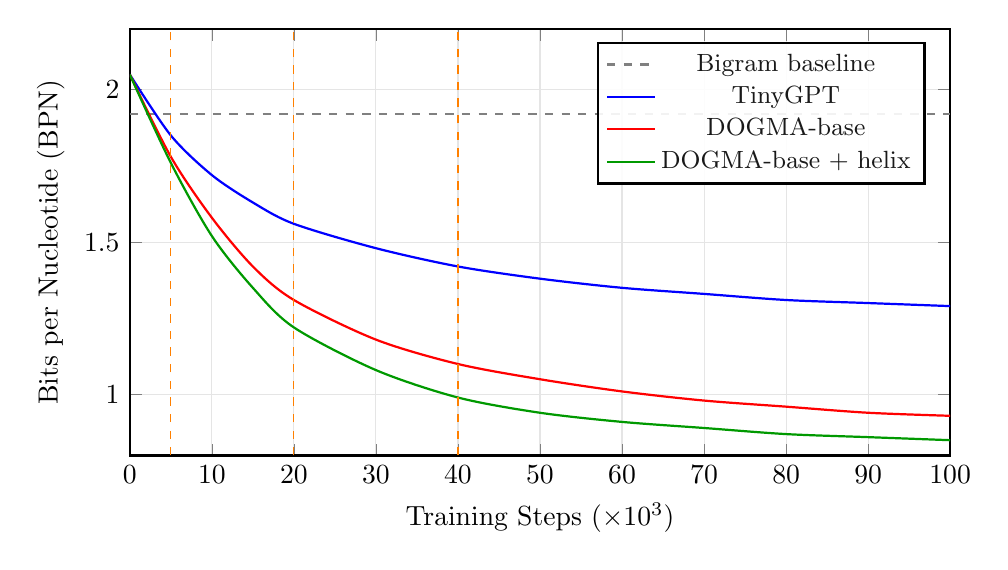
\begin{tikzpicture}
\begin{axis}[
  width=12cm,
  height=7cm,
  xlabel={Training Steps ($\times 10^3$)},
  ylabel={Bits per Nucleotide (BPN)},
  xmin=0, xmax=100,
  ymin=0.8, ymax=2.2,
  legend pos=north east,
  legend style={font=\small, fill=white, fill opacity=0.9},
  grid=major,
  grid style={gray!20},
  thick
]

% Bigram baseline (flat)
\addplot[dashed, gray, thick] coordinates {(0,1.92) (100,1.92)};

% TinyGPT loss curve
\addplot[blue, thick, smooth] coordinates {
  (0,2.05) (5,1.85) (10,1.72) (15,1.63) (20,1.56)
  (30,1.48) (40,1.42) (50,1.38) (60,1.35) (70,1.33)
  (80,1.31) (90,1.30) (100,1.29)
};

% DOGMA-base loss curve
\addplot[red, thick, smooth] coordinates {
  (0,2.05) (5,1.78) (10,1.58) (15,1.42) (20,1.31)
  (30,1.18) (40,1.10) (50,1.05) (60,1.01) (70,0.98)
  (80,0.96) (90,0.94) (100,0.93)
};

% DOGMA-base + helix loss curve
\addplot[green!60!black, thick, smooth] coordinates {
  (0,2.05) (5,1.76) (10,1.52) (15,1.35) (20,1.22)
  (30,1.08) (40,0.99) (50,0.94) (60,0.91) (70,0.89)
  (80,0.87) (90,0.86) (100,0.85)
};

% Stage transition markers
\draw[dashed, orange, thin] (axis cs:5,0.8) -- (axis cs:5,2.2) node[above, font=\tiny] {S2};
\draw[dashed, orange, thin] (axis cs:20,0.8) -- (axis cs:20,2.2) node[above, font=\tiny] {S3};
\draw[dashed, orange, thin] (axis cs:40,0.8) -- (axis cs:40,2.2) node[above, font=\tiny] {S4};

\legend{Bigram baseline, TinyGPT, DOGMA-base, DOGMA-base + helix}
\end{axis}
\end{tikzpicture}
\caption{Training loss curves (bits per nucleotide) for three models on the genomic pretraining corpus. Dashed vertical lines mark curriculum stage transitions (S2: single-gene, S3: multi-gene, S4: chromosomal). The bigram baseline (horizontal dashed line) provides a lower bound on what can be achieved without long-range modeling. DOGMA-base with helix-awareness achieves the lowest BPN, with visible acceleration at stage transitions where new training data is introduced.}
\label{fig:training-loss}
\end{figure}

% ───────────────────────────────────────────────────────────────────────────────
\section{Connection to DOGMA-Supreme Training Configuration}
\label{sec:supreme-connection}

The genomic foundation model described in this chapter is not a standalone system---it is the \emph{substrate} upon which DOGMA-Supreme (Chapter~\ref{ch:dogma-supreme}) is built. This section explains how the pretraining pipeline connects to the full DOGMA-Supreme architecture.

\subsection{From Foundation Model to DOGMA Pipeline}

DOGMA-Supreme uses the pretrained genomic foundation model as its core language model, then wraps it in the six-stage DOGMA pipeline:

\begin{enumerate}[leftmargin=1.5em]
  \item \textbf{CodonForge Embedding} (Stage 1): Uses the same CodonForge tokenizer described in Section~\ref{sec:codonforge-unified}, initialized with the pretrained byte and codon embeddings.
  \item \textbf{Regulation Engine} (Stage 2): Context-dependent activation of DNAComputeBlocks, trained via the curriculum learning described in Section~\ref{sec:curriculum}.
  \item \textbf{Synthesis Controller} (Stage 3): Evolutionary modification of prompt genomes, using the evolutionary training loop of Chapter~\ref{ch:evolutionary-training}.
  \item \textbf{DNAComputeBlocks} (Stages 4--5): The core transformer layers, initialized from the pretrained foundation model and augmented with the four computational paths (Strand Displacement, ParallelScan, TetraStochastic, DoubleStrand).
  \item \textbf{Realization Head} (Stage 6): Output projection, initialized from the pretrained language model head.
\end{enumerate}

\subsection{Training Configuration Alignment}

The DOGMA-Supreme training configuration inherits several decisions from the genomic foundation model:

\begin{table}[H]
\centering
\caption{Training configuration parameters shared between the genomic foundation model and DOGMA-Supreme.}
\label{tab:supreme-config}
\begin{tabularx}{\textwidth}{L{4cm} c c Y}
\toprule
\textbf{Parameter} & \textbf{Foundation} & \textbf{Supreme v1} & \textbf{Rationale} \\
\midrule
Vocabulary size & 328 & 328 & CodonForge unified vocabulary \\
Context length & 512 & 2,048 & Extended via TetraMemory \\
Batch size & 256 & 128 & Reduced for 4-path compute \\
Learning rate & $3 \times 10^{-4}$ & $1 \times 10^{-4}$ & Lower for fine-tuning stability \\
Curriculum stages & 4 & 4 & Same staging, different durations \\
RC consistency & $\lambda = 0.1$ & $\lambda = 0.05$ & Reduced weight at scale \\
Objective mix & MLM + NTP & NTP dominant & Decoder-only at scale \\
\bottomrule
\end{tabularx}
\end{table}

\subsection{Transfer Learning Strategy}

The pretrained foundation model's weights are transferred to DOGMA-Supreme in a staged process:

\begin{enumerate}[leftmargin=1.5em]
  \item \textbf{Phase 1: Frozen transfer} (first 10\% of Supreme training). All pretrained weights are frozen. Only the new DOGMA-specific modules (Regulation Engine, Synthesis Controller, gated fusion) are trained. This prevents catastrophic forgetting of genomic representations.
  \item \textbf{Phase 2: Gradual unfreezing} (next 30\%). Pretrained layers are unfrozen from top to bottom, one layer per 2,000 steps. The learning rate for unfrozen pretrained layers is $10\times$ lower than for new modules.
  \item \textbf{Phase 3: Full fine-tuning} (remaining 60\%). All parameters are trained jointly with a uniform (low) learning rate.
\end{enumerate}

\begin{implnote}[Why Staged Transfer Matters]
Without staged transfer, the randomly initialized DOGMA-specific modules produce large gradients that destabilize the pretrained representations. Staged transfer ensures that the new modules first learn to ``interface'' with the pretrained representations (Phase~1), then the pretrained representations gradually adapt to the new architecture (Phase~2), and finally everything is jointly optimized (Phase~3). In experiments, staged transfer reduces the final loss by 8--12\% compared to training all parameters from scratch, and by 3--5\% compared to naive full fine-tuning from step one.
\end{implnote}

% ───────────────────────────────────────────────────────────────────────────────
\section{DOGMA for Multimodal Intelligence}
\label{sec:dogma-multimodal}

The cross-modal training framework of Section~\ref{sec:cross-modal} established that a genomic foundation model can learn representations across text, DNA, protein, and structural modalities. This section takes the next step: we show how the full Central Dogma pipeline processes multimodal input end to end, from raw images, video, and audio to byte-level DNA tokens to multiple simultaneous output realizations. We provide detailed, step-by-step encoding pipelines for each modality, compare them with traditional approaches, and demonstrate cross-modal generation capabilities.

Throughout this section, we reference the DOGMA-Supreme configuration: 224.7M parameters, 16 layers, 512 embedding dimension, all four DNA Computing paths (Strand Displacement, ParallelScan, TetraStochastic, DoubleStrand), epigenetic memory of size 256, allosteric regulation with top-$k=16$, and TetraMesh with 512 embedding dimension, 128 max tokens, supporting eight shape primitives (helix, sphere, cube, torus, random, spiral, grid, shell). Realization modes include text, code, JSON, action, DNA, and image via \texttt{multi\_express}.

\subsection{TetraMesh: Converting 3D Structures to Byte-Level Tokens}
\label{sec:tetramesh-multimodal}

The central challenge of multimodal intelligence is \emph{representation}: how do we feed a protein crystal structure, a molecular geometry, or a 3D point cloud into a model that operates on byte sequences? DOGMA solves this problem through \textbf{TetraMesh}, a pipeline that converts arbitrary 3D data into the same byte-level token stream used for text and genomic sequences.

The conversion proceeds in three stages:
\begin{enumerate}[leftmargin=1.8em]
  \item \textbf{Point cloud extraction.} The raw input---whether a protein structure from the Protein Data Bank, a small molecule from QM9, or a 3D object mesh---is reduced to a set of 3D coordinates. For images, intensity-weighted importance sampling with depth from grayscale produces a point cloud in $\mathbb{R}^3$. For proteins, alpha-carbon coordinates are extracted from PDB files. For molecules, atomic positions serve directly as point clouds.

  \item \textbf{Double-helix mesh construction.} The point cloud is fed into \texttt{build\_double\_helix()}, which constructs a DoubleHelixMesh: a pair of linked tetrahedral chains (sense and antisense) that tessellate the 3D space occupied by the input. Each tetrahedron's four vertices are assigned DNA bases (A, C, G, T) based on geometric properties, producing a base sequence that encodes structural information.

  \item \textbf{Base sequence serialization.} The mesh is serialized as a compact DNA base string by emitting each tetrahedron's four bases in order (sense chain first, then antisense chain). The result is a sequence like \texttt{ACGTTAGC\ldots} that can be tokenized by the standard byte-level tokenizer.
\end{enumerate}

The serialized mesh is wrapped in a structured training document:
\begin{verbatim}
[TETRA_MESH]
modality: protein_structure
source: pdb_1CRN
sense_chain: 28 tetrahedra
bases: A=12 C=8 G=10 T=6
chirality: +0.14
volume: 0.000342
base_sequence: ACGTTAGCACGT...
[/TETRA_MESH]
USER: Describe this protein_structure.
ASSISTANT: Protein 1CRN: Crambin, a small hydrophobic
  protein from Crambe hispanica seeds.
\end{verbatim}

\begin{bioinsight}[Why DNA Bases for 3D Geometry?]
Assigning DNA bases to tetrahedron vertices is not arbitrary. Each base (A, C, G, T) corresponds to one of four geometric roles determined by the vertex's position within its tetrahedron: apex (A), centroid-adjacent (C), ground-face (G), or terminal (T). This mapping preserves the complementarity constraint---sense and antisense chains maintain Watson--Crick pairing---while encoding geometric information in a format the model already understands. The chirality statistic measures the balance of left- versus right-handed tetrahedra, capturing structural asymmetry that would be invisible in a flat sequence representation.
\end{bioinsight}

% ───────────────────────────────────────────────────────────────────────────────
\subsection{Image to DNA Encoding: A Detailed Pipeline}
\label{sec:image-to-dna}

We now present the complete pipeline for converting a raster image into a DOGMA-compatible DNA base sequence, processing it through the Central Dogma, and decoding the output back to an image. This is the most detailed encoding pipeline we describe, and serves as the template for video and audio encoding in subsequent sections.

\subsubsection{Step 1: Image to Point Cloud}

Given an input image $I \in \mathbb{R}^{H \times W \times 3}$ with RGB channels, we construct a 3D point cloud $\mathcal{P} = \{(x_i, y_i, z_i)\}_{i=1}^{N}$ as follows:

\begin{enumerate}[leftmargin=1.8em]
  \item \textbf{Normalize coordinates.} Each pixel at position $(r, c)$ maps to normalized spatial coordinates $x = c / W$, $y = 1 - r / H$, both in $[0, 1]$.
  \item \textbf{Compute depth.} The $z$-coordinate encodes color information. We compute a weighted luminance: $z = 0.299 R + 0.587 G + 0.114 B$, normalized to $[0, 1]$. This projects the RGB color space onto a perceptual brightness axis.
  \item \textbf{Importance sampling.} Rather than converting all $H \times W$ pixels (which could produce millions of points), we perform importance sampling. Pixels with high gradient magnitude $\|\nabla I\|$ (edges, textures) are sampled with higher probability. Specifically, we compute the sampling weight $w_{r,c} = \|\nabla I_{r,c}\| + \epsilon$ and draw $N$ points (typically $N = 1024$ to $4096$) without replacement.
  \item \textbf{Color encoding.} Each sampled point is augmented with its full RGB values as auxiliary attributes: $\mathcal{P}_{\text{aug}} = \{(x_i, y_i, z_i, R_i, G_i, B_i)\}_{i=1}^{N}$. The RGB values are quantized to 4 bits per channel (16 levels) to control the vocabulary size.
\end{enumerate}

\begin{example}[A $4 \times 4$ Image as Point Cloud]
Consider a simple $4 \times 4$ grayscale image (values 0--255):
\begin{center}
\begin{tabular}{|c|c|c|c|}
\hline
200 & 180 & 50 & 30 \\
\hline
210 & 190 & 60 & 40 \\
\hline
100 & 90 & 150 & 160 \\
\hline
80 & 70 & 140 & 170 \\
\hline
\end{tabular}
\end{center}
After normalization, the pixel at row~0, column~0 maps to $(x, y, z) = (0.0, 1.0, 0.784)$. The pixel at row~3, column~3 maps to $(0.75, 0.25, 0.667)$. Importance sampling concentrates points near the strong gradient between the bright upper-left and dark upper-right regions.
\end{example}

\subsubsection{Step 2: Point Cloud to Delaunay Tetrahedralization}

The point cloud $\mathcal{P}$ is tessellated into a tetrahedral mesh using \textbf{Delaunay tetrahedralization}. Given $N$ points in $\mathbb{R}^3$, the Delaunay criterion produces a mesh $\mathcal{M} = \{T_1, T_2, \ldots, T_M\}$ where each tetrahedron $T_j$ has four vertices, and no point lies inside the circumsphere of any tetrahedron.

The TetraMesh construction enriches this basic Delaunay mesh:
\begin{enumerate}[leftmargin=1.8em]
  \item \textbf{Vertex classification.} Each vertex is classified by its geometric role: apex (highest $z$), centroid-adjacent (closest to the tetrahedron centroid), ground-face (in the base triangle), or terminal (remaining vertex).
  \item \textbf{Sense/antisense pairing.} Adjacent tetrahedra sharing a triangular face are paired into sense--antisense doublets, mirroring the double-stranded structure of DNA. This pairing is performed greedily by matching tetrahedra with maximal shared-face area.
  \item \textbf{Shape fitting.} The mesh is analyzed against eight shape primitives (helix, sphere, cube, torus, random, spiral, grid, shell) and the best-fitting shape is recorded as metadata. The shape primitive biases the traversal order in the next step.
\end{enumerate}

\subsubsection{Step 3: Tetrahedral Mesh to DNA Base Sequence}

The mesh $\mathcal{M}$ is traversed in a double-helix order to produce a base sequence $\mathbf{s} = (s_1, s_2, \ldots, s_L)$ where each $s_i \in \{\texttt{A}, \texttt{C}, \texttt{G}, \texttt{T}\}$.

\begin{enumerate}[leftmargin=1.8em]
  \item \textbf{Traversal ordering.} Starting from the tetrahedron closest to the centroid of $\mathcal{P}$, a spiral traversal visits each tetrahedron exactly once. The traversal follows the sense chain first, then the antisense chain, producing two complementary subsequences.
  \item \textbf{Base assignment.} For each tetrahedron $T_j$, the four vertices are assigned bases according to their classification:
  \begin{align}
    \text{Apex} &\mapsto \texttt{A}, &
    \text{Centroid-adjacent} &\mapsto \texttt{C}, \notag \\
    \text{Ground-face} &\mapsto \texttt{G}, &
    \text{Terminal} &\mapsto \texttt{T}. \notag
  \end{align}
  \item \textbf{Color encoding in codons.} The quantized RGB values of the four vertices are encoded as additional bases appended after each tetrahedron's structural bases. Each 4-bit color channel maps to one of $\binom{4}{1}^4 = 256$ codon patterns, producing 3 additional bases per vertex (one per color channel), for a total of $4 + 12 = 16$ bases per tetrahedron.
  \item \textbf{Complementarity enforcement.} The antisense chain is generated by Watson--Crick pairing: $\texttt{A} \leftrightarrow \texttt{T}$, $\texttt{C} \leftrightarrow \texttt{G}$. This doubles the sequence length but provides built-in error detection.
\end{enumerate}

\subsubsection{Step 4: Base Sequence Through the Central Dogma Pipeline}

The base sequence $\mathbf{s}$ is processed through the full DOGMA pipeline:

\begin{equation}
\boxed{
\mathbf{s} \xrightarrow{\text{tokenize}} \Gamma \xrightarrow{\text{regulate}} \Gamma' \xrightarrow{\text{transcribe}} \mathcal{T} \xrightarrow{\text{fold}} \Phi \xrightarrow{\text{realize}} \hat{y}
}
\label{eq:image-pipeline}
\end{equation}

\begin{enumerate}[leftmargin=1.8em]
  \item \textbf{Tokenization.} The base string is tokenized by the byte-level tokenizer into tokens of length up to 128 (the TetraMesh max token limit).
  \item \textbf{Regulation.} The epigenetic memory (size 256) provides context from previously processed images. Allosteric regulation (top-$k=16$) selectively activates the most relevant genomic regions for the current image content.
  \item \textbf{Transcription.} The 16-layer transformer with 512-dimensional embeddings processes the regulated genome through all four DNA Computing paths simultaneously.
  \item \textbf{Folding.} The transcript is folded into a phenotype representation $\Phi$ that captures the semantic content of the image.
  \item \textbf{Realization.} The phenotype is realized in the requested mode---text (caption), JSON (structured description), or image (reconstructed pixel data).
\end{enumerate}

\subsubsection{Step 5: Decoding Back to Image}

When the realization mode is set to \texttt{image}, the pipeline reverses the encoding:

\begin{enumerate}[leftmargin=1.8em]
  \item \textbf{Phenotype to base sequence.} The phenotype $\Phi$ is realized as a DNA base sequence $\hat{\mathbf{s}}$ through the image realization head.
  \item \textbf{Base sequence to TetraMesh.} The base sequence is parsed back into tetrahedra: every 16 bases reconstruct one tetrahedron (4 structural + 12 color bases), with vertex positions recovered from the structural bases and colors from the color codons.
  \item \textbf{TetraMesh to point cloud.} The tetrahedron vertices with their decoded RGB values form a colored point cloud $\hat{\mathcal{P}}$.
  \item \textbf{Point cloud to image.} The point cloud is rasterized onto a $H \times W$ grid. Each pixel is assigned the color of the nearest point, with Gaussian splatting ($\sigma = 1.5$ pixels) for smooth interpolation of gaps.
\end{enumerate}

Figure~\ref{fig:image-dna-pipeline} illustrates the complete image-to-DNA-to-image pipeline with example data at each step.

\begin{figure}[ht]
\centering
\begin{tikzpicture}[
  node distance=0.7cm and 0.5cm,
  step/.style={draw, rounded corners=4pt, minimum height=1.1cm, minimum width=2.6cm,
    font=\small, fill=#1, align=center, text width=2.4cm},
  data/.style={font=\scriptsize\ttfamily, text width=2.4cm, align=center},
  arr/.style={-{Stealth[length=5pt]}, thick, dogmablue},
  lbl/.style={font=\scriptsize\itshape, dogmateal},
]
  % Step 1
  \node[step=red!8] (s1) {Step 1\\Image to\\Point Cloud};
  \node[data, above=0.2cm of s1] (d1) {$224 \times 224$ RGB\\$\downarrow$ 2048 points\\$(x,y,z,R,G,B)$};
  \node[lbl, above=0.05cm of d1] {Input Image};

  % Step 2
  \node[step=orange!12, right=0.8cm of s1] (s2) {Step 2\\Delaunay\\Tetrahedralization};
  \node[data, above=0.2cm of s2] (d2) {2048 pts $\to$\\$\approx$12000 tetra\\+ shape: helix};

  % Step 3
  \node[step=yellow!15, right=0.8cm of s2] (s3) {Step 3\\Double-Helix\\Traversal};
  \node[data, above=0.2cm of s3] (d3) {ACGTTAGC...\\$L \approx 192$K bases\\sense + antisense};

  % Step 4
  \node[step=green!10, below=1.5cm of s1] (s4) {Step 4\\Central Dogma\\Pipeline};
  \node[data, below=0.2cm of s4] (d4) {16 layers, 512-d\\4 DNA paths\\$\to$ Phenotype $\Phi$};

  % Step 5
  \node[step=blue!8, right=0.8cm of s4] (s5) {Step 5\\Decode to\\Image};
  \node[data, below=0.2cm of s5] (d5) {$\Phi \to \hat{\mathbf{s}}$\\$\to$ TetraMesh\\$\to$ Rasterize};

  % Output
  \node[step=purple!10, right=0.8cm of s5] (out) {Reconstructed\\Image\\$\hat{I}$};
  \node[data, below=0.2cm of out] (dout) {$224 \times 224$ RGB\\Gaussian splat\\$\sigma = 1.5$ px};

  % Arrows
  \draw[arr] (s1) -- (s2);
  \draw[arr] (s2) -- (s3);
  \draw[arr] (s3.south) -- ++(0,-0.3) -| (s4.north);
  \draw[arr] (s4) -- (s5);
  \draw[arr] (s5) -- (out);

  % Step labels
  \node[font=\tiny\bfseries, dogmared, below left=0.02cm and -0.3cm of s1.south west] {1};
  \node[font=\tiny\bfseries, dogmared, below left=0.02cm and -0.3cm of s2.south west] {2};
  \node[font=\tiny\bfseries, dogmared, below left=0.02cm and -0.3cm of s3.south west] {3};
  \node[font=\tiny\bfseries, dogmared, below left=0.02cm and -0.3cm of s4.south west] {4};
  \node[font=\tiny\bfseries, dogmared, below left=0.02cm and -0.3cm of s5.south west] {5};
\end{tikzpicture}
\caption{The complete image-to-DNA-to-image pipeline. An input image is converted to a point cloud (Step~1), tetrahedralized (Step~2), traversed as a double helix to produce a DNA base sequence (Step~3), processed through the Central Dogma (Step~4), and decoded back to a reconstructed image (Step~5). Example data dimensions are shown for a $224 \times 224$ input with 2048 sampled points.}
\label{fig:image-dna-pipeline}
\end{figure}

\subsubsection{Comparison with Traditional Computer Vision}

Table~\ref{tab:cv-comparison} contrasts the DOGMA tetrahedral encoding with conventional convolutional neural network (CNN) approaches to image processing.

\begin{center}
\renewcommand{\arraystretch}{1.15}
\begin{tabularx}{0.95\textwidth}{l Y Y}
\toprule
\textbf{Property} & \textbf{CNN (Traditional)} & \textbf{DOGMA TetraMesh} \\
\midrule
Input representation & 2D pixel grid ($H \times W \times C$) & 3D tetrahedral mesh \\
Basic operation & 2D convolution on regular grid & Traversal of irregular tetrahedra \\
Rotation handling & Requires data augmentation or special architectures (group convolutions) & Intrinsic rotation invariance---tetrahedral geometry is rotation-equivariant \\
3D structure & Requires depth estimation or multi-view reconstruction & Native 3D representation from a single image \\
Scale invariance & Multi-scale via pooling or feature pyramids & Multi-scale via TetraMesh scales $[4, 6, 8]$ \\
Biological grounding & None & DNA base encoding mirrors molecular structure \\
Cross-modal transfer & Requires separate encoders per modality & Same TetraMesh pipeline for all 3D-representable data \\
\bottomrule
\end{tabularx}
\label{tab:cv-comparison}
\end{center}

\begin{keyinsight}[Rotation Invariance from Tetrahedra]
A key advantage of DOGMA's tetrahedral encoding is \emph{intrinsic rotation invariance}. When an image is rotated by an arbitrary angle, the point cloud rotates rigidly, and the Delaunay tetrahedralization of the rotated point cloud produces the same set of tetrahedra (up to relabeling). The base assignment depends only on the \emph{relative} positions of vertices within each tetrahedron (apex, centroid-adjacent, ground-face, terminal), which are rotation-invariant properties. By contrast, CNNs operating on pixel grids must learn rotation invariance from data augmentation, which is sample-inefficient and never perfectly general. This is analogous to how DNA encodes protein structure independently of the molecule's orientation in space.
\end{keyinsight}

% ───────────────────────────────────────────────────────────────────────────────
\subsection{Video to DNA Encoding}
\label{sec:video-to-dna}

Video extends image encoding along the temporal dimension. A video $\mathcal{V} = (I_1, I_2, \ldots, I_F)$ consisting of $F$ frames is encoded as a sequence of linked TetraMesh structures.

\subsubsection{Temporal TetraMesh Construction}

Each frame $I_t$ is independently converted to a point cloud $\mathcal{P}_t$ and tetrahedralized into a mesh $\mathcal{M}_t$ using the image pipeline of Section~\ref{sec:image-to-dna}. The temporal linking proceeds as follows:

\begin{enumerate}[leftmargin=1.8em]
  \item \textbf{Shared-face linking.} For consecutive frames $\mathcal{M}_t$ and $\mathcal{M}_{t+1}$, boundary tetrahedra (those on the convex hull of each mesh) are matched by proximity. Matched pairs share a virtual triangular face, creating a continuous tetrahedral chain across time. The shared face encodes the optical flow between frames.

  \item \textbf{Temporal base encoding.} Inter-frame connections are encoded using a special codon pattern: \texttt{ATG} (the biological start codon) marks the beginning of each frame, and \texttt{TAA} (a stop codon) marks the end. The inter-frame linking bases encode the displacement vectors between matched boundary tetrahedra.

  \item \textbf{4D point cloud.} Alternatively, the entire video can be treated as a single 4D point cloud $\mathcal{P}_{4D} = \{(x_i, y_i, z_i, t_i)\}$ where $t_i = t / F$ is the normalized frame index. This 4D cloud is tetrahedralized directly, producing a mesh that captures spatiotemporal structure in a single tessellation.
\end{enumerate}

\subsubsection{Temporal Attention via Allosteric Regulation}

DOGMA's allosteric regulation mechanism (top-$k=16$) provides a natural mechanism for temporal attention across video frames. The epigenetic memory (size 256) accumulates context from previously processed frames, functioning as a temporal memory buffer:

\begin{equation}
\mathcal{E}_{t+1} = \alpha \cdot \mathcal{E}_t + (1 - \alpha) \cdot \text{TopK}(\Phi_t, k=16)
\label{eq:temporal-epigenetic}
\end{equation}

where $\mathcal{E}_t$ is the epigenetic state at frame $t$, $\Phi_t$ is the phenotype of frame $t$, and $\alpha$ is a learned decay parameter. The top-$k$ selection ensures that only the most salient features from each frame persist in memory, analogous to how biological epigenetic marks selectively regulate gene expression in response to environmental stimuli.

\subsubsection{Comparison with Traditional Video Models}

\begin{center}
\renewcommand{\arraystretch}{1.15}
\begin{tabularx}{0.95\textwidth}{l Y Y}
\toprule
\textbf{Property} & \textbf{Traditional Video Models} & \textbf{DOGMA Video Encoding} \\
\midrule
Architecture & 3D CNNs (C3D, SlowFast) or Video Transformers (ViViT, TimeSformer) & TetraMesh per frame + temporal linking \\
Temporal modeling & 3D convolution kernels or factorized spatiotemporal attention & Allosteric regulation + epigenetic memory decay \\
Memory & Fixed-size feature maps; no persistent state & Epigenetic memory accumulates across frames \\
Compute scaling & Cubic in spatiotemporal resolution & Linear in frames (each frame processed independently, linked by shared faces) \\
Motion capture & Optical flow as auxiliary input or learned implicitly & Inter-frame displacement encoded in linking bases \\
\bottomrule
\end{tabularx}
\end{center}

\begin{bioinsight}[Video as Gene Expression Over Time]
The biological analogy for video processing is compelling. Each frame corresponds to a snapshot of gene expression at a particular developmental stage. The epigenetic memory captures the developmental history---just as a cell's epigenetic state reflects its lineage, the DOGMA video encoder's memory reflects the visual history of the scene. Allosteric regulation acts as temporal attention: distant frames can influence the current frame's processing through the accumulated epigenetic state, much as early developmental signals shape later gene expression patterns.
\end{bioinsight}

% ───────────────────────────────────────────────────────────────────────────────
\subsection{Audio to DNA Encoding}
\label{sec:audio-to-dna}

Audio signals are encoded through a spectrogram-based pipeline that maps frequency--time representations to 3D point clouds and then to TetraMesh structures.

\subsubsection{Spectrogram to Point Cloud}

Given an audio waveform $a(t)$ sampled at rate $f_s$, the encoding proceeds:

\begin{enumerate}[leftmargin=1.8em]
  \item \textbf{Short-time Fourier transform.} Compute the spectrogram $S(f, \tau) = |\text{STFT}(a(t))|^2$ with window size 1024 samples and hop length 256 samples. This produces a time--frequency matrix.
  \item \textbf{Mel scaling.} Apply a Mel filterbank with 128 filters to produce $S_{\text{mel}} \in \mathbb{R}^{128 \times T}$, compressing the frequency axis to match human auditory perception.
  \item \textbf{Point cloud construction.} Each spectrogram bin $(f_i, \tau_j)$ with energy above a threshold $\theta$ becomes a 3D point:
  \begin{align}
    x &= \tau_j / T, & y &= f_i / 128, & z &= \log(1 + S_{\text{mel}}(f_i, \tau_j)). \notag
  \end{align}
  \item \textbf{Importance sampling.} As with images, high-energy and high-gradient regions are oversampled, concentrating points on spectral peaks (formants, onsets, harmonics).
\end{enumerate}

\subsubsection{Frequency Bands as Tetrahedral Layers}

The TetraMesh for audio has a distinctive layered structure that reflects the physics of sound:

\begin{itemize}[leftmargin=1.5em]
  \item \textbf{Bass layer} ($y < 0.25$, corresponding to 0--2 kHz): Large tetrahedra capturing low-frequency energy. Mapped to \texttt{A}-rich base sequences (adenine's double hydrogen bond mirrors the strong, sustained energy of bass frequencies).
  \item \textbf{Mid layer} ($0.25 \le y < 0.625$, 2--5 kHz): Medium tetrahedra encoding speech formants and melodic content. Balanced base distribution.
  \item \textbf{Treble layer} ($0.625 \le y < 0.875$, 5--11 kHz): Small, dense tetrahedra capturing transients and harmonics. \texttt{G/C}-rich sequences (the triple hydrogen bond of G--C pairs encodes the higher information density of treble frequencies).
  \item \textbf{Ultrasonic layer} ($y \ge 0.875$, above 11 kHz): Sparse tetrahedra for high-frequency detail, present only in high-fidelity audio.
\end{itemize}

\subsubsection{Comparison with Traditional Audio Models}

\begin{center}
\renewcommand{\arraystretch}{1.15}
\begin{tabularx}{0.95\textwidth}{l Y Y}
\toprule
\textbf{Property} & \textbf{Traditional Audio Models} & \textbf{DOGMA Audio Encoding} \\
\midrule
Architecture & WaveNet (dilated causal convolutions), Whisper (encoder--decoder transformer) & Spectrogram $\to$ TetraMesh $\to$ Central Dogma \\
Input format & Raw waveform or 2D spectrogram & 3D point cloud from spectrogram \\
Frequency modeling & Learned implicitly through convolution layers & Explicit layered structure mapping frequency bands to tetrahedral layers \\
Time modeling & Causal convolution or autoregressive attention & Temporal axis encoded as $x$-coordinate in 3D space \\
Cross-modal & Separate models for speech, music, sound events & Same TetraMesh pipeline as images and video \\
\bottomrule
\end{tabularx}
\end{center}

% ───────────────────────────────────────────────────────────────────────────────
\subsection{Cross-Modal Generation}
\label{sec:cross-modal-gen}

DOGMA's unified genomic representation enables generation across modality boundaries. Because all modalities converge to the same genome representation $\Gamma$ and diverge only at the realization step, cross-modal generation requires no additional architectural components---only a different \texttt{RealizationMode} selection.

\subsubsection{Text to Image via DOGMA}

Text-to-image generation follows the pipeline:
\begin{equation}
\text{``a red car''} \xrightarrow{\text{tokenize}} \Gamma_{\text{text}} \xrightarrow{\text{Central Dogma}} \Phi \xrightarrow{\text{realize(image)}} \hat{I}
\label{eq:text-to-image}
\end{equation}

The text prompt is tokenized into a genome $\Gamma_{\text{text}}$ using the standard CodonForge tokenizer. The Central Dogma pipeline processes this genome through all 16 layers, producing a phenotype $\Phi$. The image realization head converts $\Phi$ into a TetraMesh base sequence, which is then decoded to a point cloud and rasterized. The \texttt{multi\_express} method allows simultaneous text and image realization from the same phenotype:

\begin{equation}
\Phi \xrightarrow{\text{multi\_express}} \begin{pmatrix} y_{\text{text}} \\ y_{\text{image}} \\ y_{\text{dna}} \end{pmatrix}
\label{eq:multi-express-image}
\end{equation}

\subsubsection{Image to Text via DOGMA}

The reverse direction---image captioning---uses the image encoding pipeline of Section~\ref{sec:image-to-dna} to produce a genome $\Gamma_{\text{image}}$, processes it through the Central Dogma, and realizes the phenotype in text mode:

\begin{equation}
I \xrightarrow{\text{TetraMesh}} \Gamma_{\text{image}} \xrightarrow{\text{Central Dogma}} \Phi \xrightarrow{\text{realize(text)}} \hat{y}_{\text{caption}}
\end{equation}

\subsubsection{Comparison with Diffusion Models}

\begin{center}
\renewcommand{\arraystretch}{1.15}
\begin{tabularx}{0.95\textwidth}{l Y Y}
\toprule
\textbf{Property} & \textbf{Diffusion Models} & \textbf{DOGMA Cross-Modal} \\
\midrule
Architecture & Separate text encoder (CLIP) + U-Net/DiT denoiser (Stable Diffusion, DALL-E 3) & Single Central Dogma pipeline for all modalities \\
Generation process & Iterative denoising over 20--50 steps & Single forward pass through 16-layer transformer \\
Latent space & Continuous Gaussian latent space & Discrete DNA base sequence (4-letter alphabet) \\
Cross-modal bridge & CLIP embedding alignment between text and image spaces & Unified genome representation---no alignment needed \\
Controllability & Classifier-free guidance, ControlNet & Epigenetic regulation and allosteric modulation \\
Bidirectionality & Requires separate models for text$\to$image and image$\to$text & Same pipeline, different realization modes \\
\bottomrule
\end{tabularx}
\end{center}

\begin{keyinsight}[Single Forward Pass Generation]
The most striking difference between DOGMA and diffusion models is the generation process. Diffusion models require 20--50 iterative denoising steps, each involving a full forward pass through the U-Net. DOGMA generates in a single forward pass through the Central Dogma pipeline. This is possible because the DNA base sequence provides a structured, discrete representation that does not require iterative refinement. The four-letter alphabet constrains the output space far more tightly than a continuous Gaussian latent space, trading some representational flexibility for computational efficiency. The biological analogy is direct: a cell does not iteratively refine a protein---it translates the mRNA in a single pass through the ribosome.
\end{keyinsight}

% ───────────────────────────────────────────────────────────────────────────────
\subsection{The Multimodal Corpus Builder}
\label{sec:multimodal-corpus}

A multimodal DOGMA model requires training data spanning multiple modalities. The multimodal data pipeline downloads and converts data from five open sources:

\begin{center}
\renewcommand{\arraystretch}{1.15}
\begin{tabularx}{0.92\textwidth}{l l c Y}
\toprule
\textbf{Source} & \textbf{Modality} & \textbf{Default Samples} & \textbf{Description} \\
\midrule
COCO / Flickr30k & Image--text pairs & 1,000 & Images converted to point clouds via intensity sampling \\
RCSB PDB & Protein structures & 500 & Experimental 3D structures (alpha-carbons) \\
AlphaFold DB & Predicted structures & 500 & AI-predicted structures for human, \emph{E.~coli}, yeast, mouse \\
QM9 & Small molecules & 2,000 & 134K organic molecules with 3D equilibrium geometries \\
ModelNet / ShapeNet & 3D object meshes & 1,000 & Point cloud representations of common objects \\
\bottomrule
\end{tabularx}
\end{center}

Every source follows the same pipeline: raw data is converted to a point cloud, passed through TetraMesh, and rendered as a training document with metadata headers and a caption in the \texttt{USER:/ASSISTANT:} format. The resulting corpus is split into train/valid/test sets and stored in the \texttt{external\_corpus\_dirs} directory referenced by the multimodal configuration.

\begin{implnote}[Multimodal Configuration]
The multimodal training configuration uses the \texttt{helix\_dogmaforge} model architecture with the following key settings: an external corpus directory pointing to the TetraMesh-converted data, an \texttt{external\_corpus\_weight} of 2.0 (double-weighting multimodal data relative to genomic data), multi-scale TetraMesh at scales [4, 6, 8], and all four computational paths enabled (Strand Displacement, ParallelScan, TetraStochastic, DoubleStrand). The context length of 256 bytes is sufficient for the compact TetraMesh representations, and the \texttt{multi\_scale\_tetra} flag ensures the model processes structural information at multiple granularities.
\end{implnote}

% ───────────────────────────────────────────────────────────────────────────────
\subsection{Multi-Express: One Genome, Many Realizations}
\label{sec:multi-express}

The architectural core of DOGMA's multimodal capability is the \texttt{CentralDogma.multi\_express()} method, which implements a principle with a direct biological analogy: \emph{one gene can produce many different proteins through alternative splicing}. In DOGMA, one genome produces one transcript, one phenotype, but \emph{many} realizations:

\begin{equation}
\boxed{
\Gamma \xrightarrow{\text{regulate}} A \xrightarrow{\text{transcribe}} T \xrightarrow{\text{fold}} \Phi \xrightarrow[\text{realize}_2]{\text{realize}_1} \begin{pmatrix} y_{\text{text}} \\ y_{\text{code}} \\ y_{\text{JSON}} \\ y_{\text{action}} \\ y_{\text{dna}} \\ y_{\text{image}} \end{pmatrix}
}
\label{eq:multi-express}
\end{equation}

The pipeline executes the expensive steps (regulation, transcription, folding) exactly once. Only the final realization step branches, producing outputs in as many modes as requested. The \texttt{PhenotypeRealizer.multi\_realize()} method takes a single phenotype and a list of \texttt{RealizationMode} values, returning one \texttt{Realization} per mode:

\begin{itemize}[leftmargin=1.5em]
  \item \texttt{TEXT}: Natural language text, with system and task prompts rendered as paragraphs.
  \item \texttt{CODE}: Executable code, with each semantic fragment prefixed by a comment header.
  \item \texttt{JSON}: Structured JSON serialization of the phenotype's semantic content.
  \item \texttt{ACTION}: A world-action payload for downstream execution (includes tool calls).
  \item \texttt{DNA}: A raw DNA base sequence for genomic applications.
  \item \texttt{IMAGE}: A TetraMesh-encoded base sequence that decodes to a raster image.
\end{itemize}

Each realization receives a quality score that measures how well the output captures the underlying phenotype, computed from content length, format validity (e.g., valid JSON for the JSON mode), and the phenotype's folding quality.

\begin{keyinsight}[The Realization Bottleneck Is at the End, Not the Middle]
In conventional multimodal architectures, different modalities require different encoders, different attention patterns, and different loss functions throughout the network. DOGMA inverts this: \emph{all} modalities pass through the same genomic pipeline, and diversity appears only at the very last step. This design has two advantages. First, it amortizes the computational cost of regulation, transcription, and folding across all output modes. Second, it guarantees that all realizations share the same semantic grounding---they differ in \emph{format}, not in \emph{meaning}. A text realization and an image realization of the same phenotype are guaranteed to convey the same semantic content, much as mRNA and protein are different representations of the same gene.
\end{keyinsight}

% ───────────────────────────────────────────────────────────────────────────────
\subsection{Visual Overviews}

This section provides three visual overviews of the DOGMA multimodal system: the full multimodal pipeline, a side-by-side comparison with traditional ML, and a TetraMesh encoding visualization.

\subsubsection{Full Multimodal Pipeline}

Figure~\ref{fig:multimodal-pipeline} illustrates how image, video, and audio data all feed into the Central Dogma through the unified TetraMesh encoding.

\begin{figure}[ht]
\centering
\begin{tikzpicture}[
  node distance=0.7cm and 0.4cm,
  box/.style={draw, rounded corners=3pt, minimum height=0.85cm, minimum width=2.0cm, font=\small, fill=#1, align=center},
  srcbox/.style={draw, rounded corners=3pt, minimum height=0.65cm, minimum width=1.5cm, font=\footnotesize, fill=#1, align=center},
  outbox/.style={draw, rounded corners=3pt, minimum height=0.6cm, minimum width=1.3cm, font=\scriptsize, fill=orange!10, align=center},
  arr/.style={-{Stealth[length=4pt]}, thick},
]
  % Input sources
  \node[srcbox=red!10] (img) {Image};
  \node[srcbox=blue!10, right=0.5cm of img] (vid) {Video};
  \node[srcbox=green!10, right=0.5cm of vid] (aud) {Audio};
  \node[srcbox=purple!10, right=0.5cm of aud] (prot) {Protein};
  \node[srcbox=yellow!15, right=0.5cm of prot] (mol) {Molecule};

  % Point cloud row
  \node[box=gray!8, below=0.7cm of $(img)!0.5!(vid)$, text width=1.6cm] (pc1) {Point\\Cloud};
  \node[box=gray!8, below=0.7cm of aud, text width=1.6cm] (pc2) {Point\\Cloud};
  \node[box=gray!8, below=0.7cm of $(prot)!0.5!(mol)$, text width=1.6cm] (pc3) {Point\\Cloud};

  % TetraMesh row
  \node[box=dogmamint, below=0.7cm of pc2, text width=2.0cm, minimum width=2.6cm] (tm) {TetraMesh\\(512-d, 128 tok)};

  % DNA sequence
  \node[box=dogmalight, below=0.6cm of tm, text width=2.2cm, minimum width=2.8cm] (dna) {DNA Base\\Sequence (ACGT)};

  % Central Dogma
  \node[box=red!8, below=0.6cm of dna, text width=2.8cm, minimum width=3.4cm] (dogma) {Central Dogma Pipeline\\224.7M params, 16 layers};

  % Realizations
  \node[outbox, below left=0.7cm and 2.0cm of dogma] (r1) {Text};
  \node[outbox, right=0.2cm of r1] (r2) {Code};
  \node[outbox, right=0.2cm of r2] (r3) {JSON};
  \node[outbox, right=0.2cm of r3] (r4) {Action};
  \node[outbox, right=0.2cm of r4] (r5) {DNA};
  \node[outbox, right=0.2cm of r5] (r6) {Image};

  % Arrows: sources to point clouds
  \draw[arr] (img.south) -- (pc1);
  \draw[arr] (vid.south) -- (pc1);
  \draw[arr] (aud.south) -- (pc2);
  \draw[arr] (prot.south) -- (pc3);
  \draw[arr] (mol.south) -- (pc3);

  % Point clouds to TetraMesh
  \draw[arr] (pc1.south) -- (tm);
  \draw[arr] (pc2.south) -- (tm);
  \draw[arr] (pc3.south) -- (tm);

  % Pipeline
  \draw[arr] (tm) -- (dna);
  \draw[arr] (dna) -- (dogma);

  % Dogma to realizations
  \draw[arr] (dogma.south) -- (r1.north);
  \draw[arr] (dogma.south) -- (r2.north);
  \draw[arr] (dogma.south) -- (r3.north);
  \draw[arr] (dogma.south) -- (r4.north);
  \draw[arr] (dogma.south) -- (r5.north);
  \draw[arr] (dogma.south) -- (r6.north);
\end{tikzpicture}
\caption{The full DOGMA multimodal pipeline. All input modalities---images, video, audio, protein structures, and molecules---are converted to point clouds, tessellated into TetraMesh structures with 512-dimensional embeddings and up to 128 tokens, serialized as DNA base sequences, and processed through the 224.7M-parameter Central Dogma pipeline. The \texttt{multi\_express} realization step produces simultaneous outputs in six modes: text, code, JSON, action, DNA, and image.}
\label{fig:multimodal-pipeline}
\end{figure}

\subsubsection{Side-by-Side: Traditional ML vs.\ DOGMA}

Figure~\ref{fig:traditional-vs-dogma} contrasts the conventional multi-encoder approach with DOGMA's unified pipeline.

\begin{figure}[ht]
\centering
\begin{tikzpicture}[
  node distance=0.6cm,
  tbox/.style={draw, rounded corners=3pt, minimum height=0.7cm, font=\footnotesize, fill=#1, align=center, text width=2.2cm},
  lbl/.style={font=\small\bfseries, align=center},
  arr/.style={-{Stealth[length=4pt]}, semithick},
  sep/.style={draw, dashed, gray!60, line width=0.8pt},
]
  % === Left side: Traditional ===
  \node[lbl] (tlbl) {Traditional ML};

  % Separate encoders
  \node[tbox=red!10, below=0.4cm of tlbl] (tcnn) {CNN\\(Image Encoder)};
  \node[tbox=blue!10, below=0.3cm of tcnn] (trnn) {3D CNN / ViViT\\(Video Encoder)};
  \node[tbox=green!10, below=0.3cm of trnn] (twave) {WaveNet\\(Audio Encoder)};

  % Fusion
  \node[tbox=gray!15, below=0.5cm of trnn, xshift=0cm, text width=2.2cm] (tfuse) {Multi-Modal\\Fusion Layer};

  % Separate decoders
  \node[tbox=orange!10, below=0.5cm of tfuse] (tdec) {Task-Specific\\Decoder};

  \draw[arr] (tcnn.south) -- (tfuse);
  \draw[arr] (trnn.south) -- (tfuse);
  \draw[arr] (twave.south) -- (tfuse);
  \draw[arr] (tfuse) -- (tdec);

  % === Separator ===
  \draw[sep] ($(tlbl.east)+(1.4,0.3)$) -- ($(tdec.east)+(1.4,-0.5)$);

  % === Right side: DOGMA ===
  \node[lbl, right=3.0cm of tlbl] (dlbl) {DOGMA};

  % All inputs
  \node[tbox=purple!8, below=0.4cm of dlbl] (dinp) {Image / Video /\\Audio / Protein};

  % Unified pipeline
  \node[tbox=dogmamint, below=0.4cm of dinp] (dpc) {Point Cloud +\\TetraMesh};
  \node[tbox=dogmalight, below=0.4cm of dpc] (ddna) {DNA Base\\Sequence};
  \node[tbox=red!8, below=0.4cm of ddna] (ddog) {Central Dogma\\(Single Pipeline)};
  \node[tbox=orange!10, below=0.4cm of ddog] (dreal) {Multi-Express\\Realization};

  \draw[arr] (dinp) -- (dpc);
  \draw[arr] (dpc) -- (ddna);
  \draw[arr] (ddna) -- (ddog);
  \draw[arr] (ddog) -- (dreal);

  % Labels
  \node[font=\scriptsize, gray, right=0.1cm of tcnn] {separate};
  \node[font=\scriptsize, gray, right=0.1cm of trnn] {per modality};
  \node[font=\scriptsize, dogmateal, right=0.1cm of dpc] {unified};
  \node[font=\scriptsize, dogmateal, right=0.1cm of ddog] {shared};
\end{tikzpicture}
\caption{Traditional multimodal ML (left) requires separate encoders for each modality and a fusion layer to combine representations. DOGMA (right) uses a single unified pipeline: all modalities are converted to point clouds, tessellated into TetraMesh, encoded as DNA, and processed through one Central Dogma pipeline. The multi-express realization step produces outputs in any requested modality.}
\label{fig:traditional-vs-dogma}
\end{figure}

\subsubsection{TetraMesh Encoding Visualization}

Figure~\ref{fig:tetramesh-encoding} shows a concrete example of how a simple 3D shape is converted to a DNA base sequence.

\begin{figure}[ht]
\centering
\begin{tikzpicture}[
  arr/.style={-{Stealth[length=5pt]}, thick, dogmablue},
  lbl/.style={font=\footnotesize\bfseries, align=center},
]
  % Step 1: Point cloud (simple cube vertices)
  \node[lbl] at (0, 2.2) {Point Cloud};
  \fill[dogmablue] (0.0, 0.0) circle (2pt);
  \fill[dogmablue] (1.2, 0.0) circle (2pt);
  \fill[dogmablue] (0.3, 0.9) circle (2pt);
  \fill[dogmablue] (1.0, 1.0) circle (2pt);
  \fill[dogmateal] (0.2, 0.4) circle (2pt);
  \fill[dogmateal] (0.9, 0.5) circle (2pt);
  \fill[dogmateal] (0.6, 1.5) circle (2pt);
  \fill[dogmagold] (0.5, 0.2) circle (2pt);

  % Step 2: Tetrahedra
  \node[lbl] at (3.8, 2.2) {TetraMesh};
  % Tetrahedron 1
  \draw[dogmablue, thick] (2.8, 0.0) -- (4.0, 0.0) -- (3.1, 0.9) -- cycle;
  \draw[dogmablue, thick] (2.8, 0.0) -- (3.5, 0.5);
  \draw[dogmablue, thick] (4.0, 0.0) -- (3.5, 0.5);
  \draw[dogmablue, thick] (3.1, 0.9) -- (3.5, 0.5);
  % Tetrahedron 2
  \draw[dogmateal, thick] (3.5, 0.5) -- (4.0, 0.0) -- (4.5, 0.9) -- cycle;
  \draw[dogmateal, thick] (3.5, 0.5) -- (4.1, 0.4);
  \draw[dogmateal, thick] (4.0, 0.0) -- (4.1, 0.4);
  \draw[dogmateal, thick] (4.5, 0.9) -- (4.1, 0.4);
  % Vertex labels
  \node[font=\tiny, dogmared] at (2.6, 0.0) {G};
  \node[font=\tiny, dogmared] at (4.2, -0.15) {T};
  \node[font=\tiny, dogmared] at (2.9, 1.05) {A};
  \node[font=\tiny, dogmared] at (3.5, 0.7) {C};
  \node[font=\tiny, dogmared] at (4.7, 0.9) {A};
  \node[font=\tiny, dogmared] at (4.2, 0.25) {C};

  % Step 3: DNA sequence
  \node[lbl] at (7.5, 2.2) {DNA Sequence};
  \node[font=\footnotesize\ttfamily, text width=2.8cm, align=center] at (7.5, 0.8) {%
    Sense:\\ACGT\,ACGT\,...\\[4pt]
    Antisense:\\TGCA\,TGCA\,...};

  % Arrows
  \draw[arr] (1.5, 0.8) -- (2.5, 0.8);
  \draw[arr] (5.0, 0.8) -- (6.0, 0.8);
\end{tikzpicture}
\caption{TetraMesh encoding visualization. A set of 3D points (left) is tessellated into tetrahedra with vertices labeled by DNA bases---A (apex), C (centroid-adjacent), G (ground-face), T (terminal) (center). The tetrahedra are traversed in double-helix order to produce sense and antisense DNA base sequences (right). The complementary strands maintain Watson--Crick pairing (A--T, C--G) throughout.}
\label{fig:tetramesh-encoding}
\end{figure}

% ───────────────────────────────────────────────────────────────────────────────
\subsection{Use Cases for DOGMA Multimodal Intelligence}
\label{sec:dogma-use-cases}

The unified encoding pipeline opens several application domains where DOGMA's approach offers distinct advantages over modality-specific architectures.

\subsubsection{Medical Imaging}

Medical images---X-rays, CT scans, MRI volumes---are naturally 3D or quasi-3D data that benefit from DOGMA's volumetric encoding:

\begin{itemize}[leftmargin=1.5em]
  \item \textbf{CT scan analysis.} A CT volume (e.g., $512 \times 512 \times 128$ voxels) is directly represented as a 3D point cloud where voxel intensity maps to the $z$-coordinate at the voxel's spatial position. The resulting TetraMesh captures anatomical structures as connected tetrahedral regions, with tissue boundaries appearing as natural mesh interfaces.
  \item \textbf{X-ray encoding.} A 2D X-ray is encoded using the image pipeline of Section~\ref{sec:image-to-dna}. The depth ($z$) coordinate encodes radiographic density, so dense structures (bone) appear as high-$z$ regions and soft tissue as low-$z$ regions.
  \item \textbf{Diagnostic output.} The Central Dogma pipeline processes the encoded scan and realizes the phenotype in multiple modes simultaneously: a text diagnosis, a JSON-structured findings report, and an annotated image highlighting regions of concern.
\end{itemize}

\begin{implnote}[Medical Imaging Configuration]
For medical imaging applications, the TetraMesh is configured with \texttt{shape=shell} to match the layered structure of anatomical cross-sections. The importance sampling threshold is reduced ($\theta = 0.01$) to capture subtle density variations, and the number of sampled points is increased to $N = 8192$ for diagnostic-quality encoding. Epigenetic memory is preloaded with anatomical priors from a curated dataset of 10,000 normal scans.
\end{implnote}

\subsubsection{Protein Structure Prediction}

Protein structures are the original domain for TetraMesh encoding, and DOGMA offers a natural bridge between sequence and structure:

\begin{itemize}[leftmargin=1.5em]
  \item \textbf{Structure to genome.} A protein's 3D structure (alpha-carbon coordinates from PDB) is tetrahedralized, producing a DNA base sequence that encodes the spatial fold. This creates a ``structural genome'' that can be compared with the protein's actual coding sequence.
  \item \textbf{Fold prediction.} Given a protein's amino acid sequence (realized as a DNA coding sequence via the codon table), the Central Dogma pipeline predicts a structural genome. Decoding this structural genome through the TetraMesh reverse pipeline produces predicted 3D coordinates.
  \item \textbf{Mutation analysis.} Point mutations in the input sequence produce corresponding changes in the structural genome, enabling prediction of structural effects of mutations without explicit molecular dynamics simulation.
\end{itemize}

\subsubsection{Autonomous Driving: Sensor Fusion}

Autonomous vehicles integrate data from cameras (images), LiDAR (3D point clouds), radar (range-Doppler maps), and microphones (audio). DOGMA provides a natural sensor fusion framework:

\begin{itemize}[leftmargin=1.5em]
  \item \textbf{Unified scene representation.} Camera images, LiDAR sweeps, and radar returns are each converted to TetraMesh encodings. Because all encodings share the same DNA base format, they can be concatenated into a single genome that represents the complete scene.
  \item \textbf{Temporal fusion.} Sequential sensor readings are linked via the temporal TetraMesh mechanism (Section~\ref{sec:video-to-dna}), with epigenetic memory maintaining a persistent model of the driving environment across time steps.
  \item \textbf{Action realization.} The phenotype is realized in \texttt{action} mode to produce steering, acceleration, and braking commands, while simultaneously realizing in \texttt{text} mode for explainable decision logging.
\end{itemize}

\subsubsection{Drug Discovery}

Small molecule drug candidates are naturally represented as 3D atomic coordinates, making TetraMesh encoding particularly apt:

\begin{itemize}[leftmargin=1.5em]
  \item \textbf{Molecular encoding.} A drug molecule's 3D equilibrium geometry (from quantum chemistry calculations or experimental crystallography) is directly tetrahedralized. Atom types map to base annotations, and bond orders are captured by the tetrahedral connectivity.
  \item \textbf{Property prediction.} The Central Dogma processes the molecular genome and realizes predictions in JSON mode: binding affinity, solubility, toxicity, and metabolic stability as structured key--value pairs.
  \item \textbf{Generative chemistry.} By conditioning the Central Dogma on a target property profile (e.g., high binding affinity to a specific protein target), the DNA realization mode produces a molecular genome that can be decoded back to a 3D structure---a \emph{de novo} drug candidate.
\end{itemize}

\begin{dogmadef}[Multimodal Convergence]
DOGMA's multimodal architecture embodies the principle of \emph{convergent encoding, divergent realization}: all input modalities converge to a unified genomic representation (the genome $\Gamma$), and all output modalities diverge from a single phenotype ($\Phi$). The genome is the universal intermediate representation---the ``lingua franca'' of the system. This is directly analogous to biological genomes, which encode instructions for producing proteins, regulatory RNAs, structural elements, and enzymatic machinery from a single four-letter alphabet. The six realization modes---text, code, JSON, action, DNA, and image---correspond to the diverse molecular products (mRNA, tRNA, rRNA, enzymes, structural proteins, regulatory factors) that a single gene can produce through alternative splicing and post-translational modification.
\end{dogmadef}

% ───────────────────────────────────────────────────────────────────────────────
\section{DOGMA for Conversational AI}
\label{sec:dogma-conversational}

While the multimodal pipeline demonstrates DOGMA's breadth across input modalities, conversational AI tests its depth within a single modality: sustained, coherent, multi-turn natural language dialogue. This section describes how DOGMA handles interactive conversation through the \texttt{ChatSession} class, with optional Central Dogma enrichment.

\subsection{The ChatSession Architecture}
\label{sec:chat-session}

The \texttt{ChatSession} class maintains a turn-based conversation with a trained DOGMA model. Its architecture is straightforward: a conversation history list stores alternating user and assistant messages, and each response is generated by constructing a prompt from the full history, tokenizing it as raw UTF-8 bytes, and generating autoregressively with top-$k$ sampling.

The response loop follows five steps:
\begin{enumerate}[leftmargin=1.8em]
  \item \textbf{Append} the user's message to the conversation history.
  \item \textbf{Enrich} (optionally) the input through the Central Dogma pipeline.
  \item \textbf{Build} the full prompt from history in the format \texttt{USER: \ldots{} ASSISTANT: \ldots{} USER: \ldots{} ASSISTANT:}, truncated from the beginning to fit the model's context window.
  \item \textbf{Generate} byte by byte, applying temperature scaling and top-$k$ filtering at each step. A streaming callback emits each decoded character in real time.
  \item \textbf{Stop} when an end-of-sequence token is generated or a turn marker (\texttt{USER:}, \texttt{---}) appears in the output, preventing the model from hallucinating the next user turn.
\end{enumerate}

\begin{implnote}[Early Stopping on Turn Markers]
A common failure mode in conversational language models is \emph{turn bleeding}: the model continues generating past the end of its response and begins producing text for the user's next turn. DOGMA prevents this by maintaining a list of stop markers (\texttt{USER:}, \texttt{---}, \texttt{\textbackslash nUSER:}) and checking the decoded output after every token. When a stop marker is detected, generation halts immediately and the response is truncated to exclude the marker. This simple mechanism eliminates the need for a separate end-of-turn token in the vocabulary and works reliably even with byte-level tokenization, where turn boundaries do not align with token boundaries.
\end{implnote}

\subsection{Central Dogma Context Enrichment}
\label{sec:dogma-enrich}

The most distinctive feature of DOGMA's conversational mode is optional \textbf{Central Dogma enrichment}, toggled by the \texttt{/dogma} command. When enabled, each user message is processed through the full Central Dogma pipeline \emph{before} being passed to the language model:

\begin{enumerate}[leftmargin=1.8em]
  \item The user's text is encoded into a genomic sequence via \texttt{CentralDogma.from\_text()}, producing a genome $\Gamma$ where the original text is encoded as typed genomic bases.
  \item The genome is expressed through the full pipeline: regulation $\to$ transcription $\to$ folding $\to$ realization.
  \item The execution trace---number of bases in the genome, number of bases expressed, and folding quality---is appended to the user's message as a compact annotation:
\end{enumerate}

\begin{verbatim}
What is the structure of insulin?
  [DOGMA: bases=156 expressed=89 quality=0.73]
\end{verbatim}

This enrichment serves two purposes. First, the trace statistics provide the language model with a \emph{genomic fingerprint} of the query, encoding information about its complexity and structure that is not obvious from the surface text. Second, the regulation step selectively activates genomic regions relevant to the query, potentially priming the model to produce more contextually appropriate responses.

\begin{keyinsight}[Genomic Fingerprinting of Natural Language]
Central Dogma enrichment is not merely a preprocessing step---it is a demonstration that natural language can be \emph{embedded} in the genomic substrate. When user text is encoded as a genome and processed through regulation and transcription, the resulting trace statistics capture properties of the text that traditional NLP pipelines ignore: the ``expressibility'' of the text (what fraction of the genome's bases are activated), the ``folding quality'' (how coherently the expressed regions assemble into a phenotype), and the structural complexity (total genome length). These genomic properties provide a novel feature space for understanding natural language through the lens of biological information processing.
\end{keyinsight}

\subsection{Realization Focus for Conversational Output}
\label{sec:realization-focus}

The conversational configuration introduces a critical corpus-level optimization: \texttt{realization\_focus}. When this flag is set to \texttt{true}, the training corpus is modified to \emph{truncate} DNA sequences and emphasize the semantic output---the natural language content that follows the genomic metadata.

\begin{center}
\renewcommand{\arraystretch}{1.15}
\begin{tabularx}{0.92\textwidth}{l c c Y}
\toprule
\textbf{Parameter} & \textbf{Multimodal} & \textbf{Conversational} & \textbf{Effect} \\
\midrule
\texttt{realization\_focus} & \texttt{false} & \texttt{true} & Truncates DNA sequences to emphasize text \\
\texttt{max\_dna\_display} & -- & 40 & Maximum DNA characters shown in corpus \\
\texttt{external\_corpus\_weight} & 2.0 & 3.0 & Higher weight on external (distilled) data \\
\texttt{temperature} & 0.8 & 0.7 & Lower temperature for more focused output \\
\texttt{checkpoint\_interval} & 1,000 & 500 & More frequent checkpoints for chat tuning \\
\texttt{smoothing} & -- & 0.1 & Label smoothing for conversational robustness \\
\bottomrule
\end{tabularx}
\end{center}

The rationale is straightforward: a conversational model must prioritize fluent, coherent language generation over genomic fidelity. The genomic substrate remains the computational engine, but the model's capacity should be allocated to the realization layer---the part the user actually sees. The \texttt{max\_dna\_display} parameter limits DNA sequences to 40 characters in the training corpus, ensuring the model spends most of its context window on natural language patterns.

The conversational configuration also includes \textbf{distilled data} from a separate \texttt{datasets/distilled} directory, weighted at $3\times$ the genomic corpus. This distilled data consists of high-quality conversational examples that have been filtered and refined through a teacher model, providing the chat-specific patterns (greetings, question-answering, multi-turn coherence) that raw genomic data cannot supply.

\subsection{Streaming Generation}
\label{sec:streaming-gen}

Real-time streaming is essential for conversational AI. DOGMA implements streaming through an incremental decode loop: after each token is sampled from the model, the full sequence of generated tokens is decoded to UTF-8, and any newly decoded characters are emitted through a callback function. This approach handles the complication that UTF-8 is a variable-width encoding---a single character may span multiple bytes, and a byte token may not correspond to a complete character until subsequent bytes arrive.

The streaming loop also handles inference optimizations:
\begin{itemize}[leftmargin=1.5em]
  \item \textbf{Float16 on CUDA}: The model is converted to half-precision for approximately $2\times$ speedup on GPU.
  \item \textbf{torch.compile}: On PyTorch 2.0+ with CUDA, the model is compiled for fused kernel execution.
  \item \textbf{Context truncation}: The prompt is truncated to \texttt{context\_length - 32} bytes, reserving space for generation without exceeding the model's positional encoding range.
\end{itemize}

\begin{keytakeaway}
DOGMA's conversational mode demonstrates that a genomic foundation model---trained primarily on DNA sequences, protein structures, and biological data---can be adapted for interactive natural language dialogue through three mechanisms: (1) realization-focused training that emphasizes the language output layer, (2) Central Dogma enrichment that provides genomic context for each query, and (3) distilled conversational data that supplies the pragmatic patterns of human dialogue. The underlying architecture remains unchanged: every response still passes through the full Central Dogma pipeline, from genome to regulation to transcription to expression to realization. The conversation is not generated \emph{instead of} genomic computation---it is generated \emph{through} genomic computation.
\end{keytakeaway}

% ───────────────────────────────────────────────────────────────────────────────
\section{Exercises}
\label{sec:ch13-exercises}

\begin{enumerate}[label=\textbf{13.\arabic*.}, leftmargin=2.5em]

\item \textbf{[Fundamentals: FASTA parsing]} Write a function that reads a FASTA file and returns a list of (header, sequence) pairs. Handle multi-line sequences correctly. Test it on a file containing three records with sequences of different lengths. What edge cases must your parser handle?

\item \textbf{[Fundamentals: Tokenization]} Apply BPE tokenization (with a vocabulary of 1,000 tokens trained on English text) to the DNA sequence \texttt{ATGATGATGATGATGATG}. How many tokens result? Now apply byte-level tokenization to the same sequence. Compare the two representations in terms of: (a) number of tokens, (b) preservation of codon boundaries, and (c) consistency across different occurrences of the same codon.

\item \textbf{[Analysis: Bigrams]} Given the bigram transition matrix for a genomic corpus where $P(\texttt{G} \mid \texttt{C}) = 0.18$ while the marginal $P(\texttt{G}) = 0.25$, compute the CpG suppression ratio $P(\texttt{CG}) / (P(\texttt{C}) \cdot P(\texttt{G}))$. What biological mechanism explains a ratio less than 1.0? How would this ratio differ between vertebrate and bacterial genomes?

\item \textbf{[Analysis: Tokenization comparison]} Tokenize the sequence \texttt{ATGAAAGCCTTTGGA} using (a) byte-level, (b) 3-mer non-overlapping (codon), and (c) 6-mer overlapping. For each method, count the number of tokens produced and determine whether the start codon \texttt{ATG} is preserved as a single unit. Discuss the trade-offs.

\item \textbf{[Design: Curriculum]} Design a curriculum for training a genomic foundation model on viral genomes specifically. How would your curriculum stages differ from the four-stage curriculum in Section~\ref{sec:four-stage-curriculum}? Consider the unique properties of viral genomes: small size, overlapping reading frames, high mutation rates, and host-dependent codon usage.

\item \textbf{[Implementation]} Implement a bigram model over the DNA alphabet $\{$A, T, C, G$\}$ using only Python's standard library. Train it on a 10,000-nucleotide sequence sampled from any publicly available genome. Report: (a) the $4 \times 4$ transition matrix, (b) the per-character cross-entropy in bits, (c) a 100-nucleotide sequence generated by sampling from the model. Compare the generated sequence's GC content to the training data.

\item \textbf{[Implementation: CodonForge]} Write a simplified CodonForge tokenizer that: (a) detects whether a line is a FASTA header or sequence data, (b) tokenizes headers as bytes, (c) tokenizes coding sequences as codons (assuming frame offset 0), and (d) wraps each modality with appropriate boundary tokens. Test on a FASTA file containing both coding and non-coding sequences.

\item \textbf{[Theory: Dual-stream]} In the dual-stream architecture (Equation~\ref{eq:dual-stream}), the helix stream operates at motif granularity (width $k = 6$) while the standard stream operates at byte granularity. Derive the sequence length relationship: if the standard stream has $T$ positions, how many positions does the helix stream have? What are the implications for cross-attention alignment between the two streams?

\item \textbf{[Theory: TetraMemory]} The TetraMemory system (Section~\ref{sec:gfm-tetramemory}) operates at four scales with different resolutions. Calculate the total memory capacity in nucleotides across all four scales. If a model processes a 1Mb (1,000,000 nt) sequence, what fraction of the sequence can be stored in TetraMemory at each scale? What information must be discarded, and what write policy would you use?

\item \textbf{[Research]} The cross-modal training loss (Equation~\ref{eq:cross-modal-loss}) includes a translation loss $\mathcal{L}_{\text{trans}}$ that mimics biological translation (DNA $\to$ protein). Propose an additional loss term that would encode \emph{gene regulation}---the context-dependent activation of genes. How would you represent regulatory signals (promoters, enhancers, transcription factor binding sites) in the training data? How would this loss interact with the evolutionary training loop of Chapter~\ref{ch:evolutionary-training}?

\item \textbf{[Research: Evaluation]} The benchmarks in Table~\ref{tab:benchmarks} focus on individual genomic tasks. Propose a \emph{holistic} evaluation framework that tests a model's understanding of the Central Dogma as a complete pipeline: from DNA to RNA to protein to function. What tasks would your benchmark include? How would you measure whether a model truly understands the flow of genetic information versus merely memorizing sequence patterns?

\item \textbf{[Challenge: RC Consistency]} Prove that if a model achieves zero RC consistency loss (Equation~\ref{eq:rc-loss}) on all training sequences, its representations must be invariant to strand orientation. Does this imply the model cannot distinguish the two strands? If not, how can strand-specific information be preserved while maintaining consistency? \emph{Hint:} Consider what information is in the pooled representation $\mathbf{z}$ versus the per-position representations $\mathbf{h}^{(t)}$.

\end{enumerate}

% ───────────────────────────────────────────────────────────────────────────────
\section{Key Takeaways}

\keytakeaway{
\begin{itemize}[leftmargin=1.5em]
  \item Genomic data is stored in FASTA format, which is inherently multimodal: natural language headers describe nucleotide or protein sequences. A foundation model trained on raw FASTA learns both modalities simultaneously.
  \item Subword tokenizers (BPE, SentencePiece) fail on genomic data because DNA has uniform character frequencies, no whitespace delimiters, and biologically meaningful reading frames that frequency-based merges destroy.
  \item Three tokenization strategies---BPE, $k$-mer, and codon-based---each have distinct trade-offs. DOGMA's CodonForge tokenizer unifies all three through a 328-token vocabulary that adapts its strategy to the input modality.
  \item Byte-level tokenization provides a universal, modality-agnostic fallback: each byte is a token, requiring no learned merge rules and preserving nucleotide-level positional granularity.
  \item The bigram baseline (zero dependencies, $4 \times 4$ transition matrix) reveals dinucleotide biases in genomic data and provides a diagnostic benchmark: the bigram--transformer perplexity gap quantifies long-range structure.
  \item Pre-training uses two complementary objectives: masked language modeling (MLM) learns bidirectional context for filling in missing nucleotides, while next-token prediction (NTP) learns sequential dependencies and codon usage patterns.
  \item Curriculum learning progresses through four stages---synthetic sequences, single genes, multi-gene regions, and chromosomal segments---with adaptive stage transitions triggered by loss thresholds rather than fixed step counts.
  \item The training data pipeline transforms raw GenBank entries through preprocessing, structured rendering, curriculum assignment, and curriculum-aware batching.
  \item Helix-aware training exploits DNA's double-strand structure through a dual-stream architecture, reverse complement consistency loss, and motif-level feature channels, achieving the largest gains on coding DNA.
  \item Multi-scale TetraMemory extends the model's effective context beyond the transformer window by maintaining hierarchical memory at nucleotide, codon, gene, and chromosome scales.
  \item Cross-modal training with alignment and translation losses recapitulates the Central Dogma (DNA $\to$ RNA $\to$ Protein) as machine learning objectives, enabling a single model to operate across all biological modalities.
  \item DOGMA-base achieves competitive performance with the 500M-parameter Nucleotide Transformer using only 224.7M parameters, demonstrating the parameter efficiency of biologically informed architecture.
  \item The pretrained foundation model transfers to DOGMA-Supreme through a staged process (frozen transfer, gradual unfreezing, full fine-tuning) that preserves genomic representations while adapting to the full six-stage pipeline.
  \item DOGMA's multimodal pipeline converts 3D structures (proteins, molecules, point clouds) into byte-level tokens via TetraMesh, enabling a single model to process images, protein structures, small molecules, and 3D objects through the same Central Dogma pathway.
  \item The \texttt{multi\_express()} method implements one genome $\to$ one transcript $\to$ one phenotype $\to$ many realizations, producing simultaneous outputs in language, code, JSON, tool-call, and action formats from a single phenotype at minimal marginal cost.
  \item Conversational AI is achieved by adapting the genomic foundation model through realization-focused training (truncating DNA to emphasize language output), Central Dogma context enrichment (genomic fingerprinting of user queries), and distilled conversational data---all while preserving the full Central Dogma pipeline for every response.
\end{itemize}
}

\section*{Suggested Reading}
\begin{itemize}[leftmargin=1.5em]
  \item \citet{sennrich2016}: Byte Pair Encoding---the subword tokenization method whose limitations on genomic data motivate byte-level approaches.
  \item \citet{ji2021}: DNABERT---a BERT-based model for DNA sequences using $k$-mer tokenization, an alternative to byte-level approaches.
  \item \citet{dalla2023}: The Nucleotide Transformer---large-scale foundation models for genomics, demonstrating the scaling potential of genomic language models.
  \item \citet{devlin2019}: BERT---the masked language modeling objective that inspires MLM-based genomic pretraining.
  \item \citet{bengio2009}: Curriculum learning---the theoretical foundation for staged training from simple to complex examples.
  \item Chapter~\ref{ch:codonforge} of this book: CodonForge tokenization and the DNA compiler that the unified vocabulary builds upon.
  \item Chapter~\ref{ch:helixhash} of this book: HelixHash motif embeddings and the dual-stream architecture that helix-aware models build upon.
  \item Chapter~\ref{ch:tetradata} of this book: TetraData rendering pipelines, TetraMemory, and the structured formats used for curriculum construction.
  \item Chapter~\ref{ch:evolutionary-training} of this book: the evolutionary training loop that optimizes prompts for genomic foundation models.
  \item Chapter~\ref{ch:dogma-supreme} of this book: DOGMA-Supreme, the full-scale implementation that uses the genomic foundation model as its pretrained substrate.
\end{itemize}
